\hypersetup{pdfborder=0 0 0}
%\vspace{10\baselineskip}


%\selectlanguage{french}


\section{Resume français}

Partie a été rédigée en anglais dans l'éventualité d'une soumission prochaine en tant qu'article....




%-------------------------------------------------------------------------------------
\section{Papier 3D}
\subsection{Review of general points about circulation at Gibraltar (intro/biblio)}

(revoir plan intro...)


The Atlantic - Mediterranean exchange occuring in the Strait of Gibraltar has been explained summarily in previous part (2D). It consists in Med waters exiting the Strait at depth as what has been dubbed the 'Mediterranean outflow' while Atl waters use this pathway to enter the Mediterranean basin at the surface.

Those Atlantic waters that enter the Mediterannean at the Strait are the principal contribution to the Med inflowing water budget, with the average transport of Atl waters at Gib being of the order of 1Sv. The net exchange itself is of the order of 0.1Sv as a positive entry for med that offsets the otherwise net evaporation occuring on the integrated surface of the Mediterranean basin \citep{bryden_1994}.
%(rough estimation volume that gets evaporated ??? faudrait voir évolution surface découverte med et si prend évaporation uniforme, combien de temps pour évaporer (1000an a vu cette valeur?)). 
Since the Med basin is otherwise a closed basin, this means that the Mediterranean waters exiting the Strait of Gibraltar are the result of the transformations of Atl waters that entered at the Strait.
More details are provided in this section on the characteristics of the Strait, the exchange and its variability and the processes that take place during it.



%(Sommaire de cette partie.... Review some aspects...., variabilty of baroclinic exchange, focus on the high frequency which involves the several mechanisms that are studied in high resolution numerical simulation in next section)



%deep convection dans le bassin ouest de la Méditerranée s’effectue en 3 phases (Naranjo2014): le pérconditionnement (la densifictaion en circulant en Med ... 
%Critère convection profonde, regarde eaux densité >1029,10kg/m³ et le MLD (mixed-layer depth) où la diffusion vertciale >0,04m2/s (Naranjo2014)
%Taux de formation eaux denses (=eaux profondes ?) en Med trouve entre 0,3 et 6 Sv(Naranjo2014)…




\subsubsection{Circulation in neighbouring areas (Cadix and Alboran)}

(de Pascual-Collar ; NAjanro 2012 ; Sanchez Garrido 2013 ;Lorente 2019 ; garcia lafuente 2017)


\textit{Atlantic side}

The surface waters that end up entering the Strait are NACW and SAW\citep{millot_2014,naranjo_2015}. They are carried by the Potrugal and Azores Current into Gib as part of the eastern branch of the north atlantic subtropical gyre \citep{barton_2001}

Below this surface circulation, can find in the Northern Atlantic the med outflow/the mediterranean watermass that was transported out of the Strait by the MEditerreanaen outflow. It first flows in the Gulf of Cadix, rotating to north due to geostrophy and flowing along the bathymetry of the continentl slope\citep{price_1993,gasser_2017} and west of the Gulf of Cadiz stabilizes to its neutral buoyancy level at 100m depth as the Mediteranean water mass\citep{price_1993}. Meddies, salty lenses of water with negative (?) vorticity able to 'survive' for years that are encountered in the open ocean, are generated along the canyons and caps encounetred by the Mediterranean outflow in the Gulf of Cadiz \citep{bashmachnikov_2015}. The mediterranean outflow itself participates in the global circulation/north atlantic overturning cirulation(?) by salinification of the overall north atlantic basin with the spreading of the mediterranean water mass in the open ocean and decaying of meddies, but also with a part of the outflow directly joining circulation at the pole \citep{price_1993,jia_2007}.


\textit{Mediterranean side}


Surafce waters exiting the Strait at the east enter the Alboran Sea as the Atlantic Jet (AJ). The ciruculation of the Alboran Sea is variable, witht the most common state having two anticyclonic gyre (Wag ans EAG), but not uncommon that only one of the two is present \citep{millot_2005}(?ou autre). The WAG is coupled to the Atlantic jet, that usually consctitutes its northern branch, however variability of the AJ due to meteorological and tidal forcing can destabilize this system \citep{sanchez-garrido_2013,lorente_2019}.

At depth, several mediterranean water masses enter the strait. In the Alboran Sea, identified are LIW (for Leventine Intermediate Water) and WMDW(West MEditerranean Deep Water), with other water masses of the western med bassin like TDW (Thryenian Deep Water) also being detected (Millot). There is a south/north repatition of those watermasses, with TDW, LIW and other intermediate waters more abundant in northern part of Alboran sea, and WMDW flowing more in south part \citep{millot_2014}. As the depth from teh Alboran to the Strait decreases, it is more difficult for the deeper WMDW to enter the strait. Mechanisms that help funnel it to the Strait itself would be important production of deep waters by the winter convection events that elevate the level of WMDW(...). But it is was also shown that strength of the WAG/gyre correlates/will command the 'efficiency' of evacuaing wmdw (ventilation...)//facilitated entry of WMDW in the Strait (Najanro 2012) facilitates the water that cross the sill by bernouilli suction effect (Najanro 2012;Kinder and Parilla 1987) (cette deuxième phrase dans partie détroit...) 

(aussi Izquierdo2019 sur MOW)
%Le renouveau des eaux profondes en Méditerranée soulève les eaux profondes d’avant, qui peuvent se retrouver aspirer par le détroit de Gibraltar, la marée favorise al ventilation de WMDW(Naranjo 2014). On choisit comme critère pour les eaux profondes les eaux dont la température potentielle est <14°C(Naranjo2014).

%Marée à Gibraltar refroidit les euax de la Mer d’Alboran (Naranjo 2014) , plus aurait effect advection de vorticité ?.. Voit transport cyclique par les ISW de chlorophylle vers l’est , fait des pulse (Bruno 2013)

\textit{Gen}

Whether look at inflowing Atl waters or outflowing Med waers (inflowing/ouflowing in regard to teh Med basin) (n fact, med outflow incorporated atl waters, and vice versa al inflow has med waters..., while the inflow and outflow retain some signature, they also incorporporate siganture of the other water masses of the exchange
L’atlantic inflow est constitué de SAW (eaux de surafce Atlantique), Naw (north-atlantic central water, signature plus importante en spring tide, petite devant les deux autres) et de MOW (med outflowing water) (Macias 2006)

outflow est composé d’eaux Med (LIW,WMDW, WIW) et d’eaux Atlantiques (Millot 2006?)
Outflow med incorpore aussi eau atl à cause mélange qui a lieu a CS/le long du chemin...(garcia lafuente 2011)   

Those are the water masses brfore the exchange, however they are not the weter masses that are ... The exchange at the strait does not conserve the T,S characteristics. Hence processes occur in the Strait itself that transform this water masses, ie mixing occurs, need to understand processes in the Strait itself.

%%%%%%%%%%%%%%%%%%%%%%%%%%%%%%%%
\subsubsection{Campagnes d'observations et simulations numériques à Gibraltar/ Observatons and siulatons of processes in the Strait of Gibraltar(avant ou après partie process etc.)}

LAIWS have long been oberved, due to their surface signature.   But sampling of the wter column also ...

Campaigns to evaluate the transport necessissate longer term monitoring, 

First campaigns were aiming to quantify teh exchange and understand better the med budget, the most extensive is  . But also observations of solitons duig this campaign, with Farmer and Armi(...) explaining how the soitons are created by the interaction of te exchange and tidal forcing. The solitons that had been seen before, but with remote sensing more observations. Only surface signel, Ponctual in situ campaigns also use veloity and hydological arking of teh solitons. observed more and more with ... (Lacombe 1988) ((((As well as the impat of those sall eneretical processes on biological tracers. plus tard)))
The (arggggg periodicity of teh exchange s wel aknowledged, means that to have a budget need long term monitoring is more difficult, wat to survey the med budget , INGRES. also try to go beyond quantifying the budget and to connect more precisely the med outflow composition.
Moorings to monitor the med outflow and try to correlate its signature with events in the mediterranean (for exemple rate of formation of WMDW and other water masses). but due to vigorous mixing, med outflow difficult to single out all contributions.(garcia lafuente 2017) region of high trafic so long term mooring difficult especially in narrower sections. 1 mouillage Espartel sill longue durée (10 ans, Sammartino 2015, INGRES)

Ziegenbein (1970) obs with moorings, obs in september 1868 with three morrings aligned from the etsern eand of the strait. 

Many simulation experiments to understand propagation of solitons. As said in part. however only non-hydrostatic models can be used. The exchange as a part of the mediterranean and north atlantic circulation is more dfficult to represent as need big grids, . 
But the narrowness of the Gibraltar Strait means it is coarsely resolved in global (or even mediterranean) models. In global models parametrized...
Also studies to represent this exchange more explicitely, For exemple the model as local rafinemnt by putting Gibraltar in 'pole' position. ... also used imbrication model.

The characteristics of the Med waters that arrive at the eastern boundary of the strait are commanded by the processes of the med sea (convection, ...). 


In climate mode, parametrised with enhanced mixing (voir refdans Sanchez ronan 2018...)

(ref après dans les auters parties?)

Campagnes et obs in situ : Gibraltar 2008 (Bruno 2013) / INGRES (mooring à ES depuis 2004) / CANIGO( 95-98) Garcia Lafuente 2002 /Vargas 2006(moorings sortie est du détroit et CS) /2 mouillages mai 2003 propagation ISW (Sanchez Garrido 2008)/Watson 1990 obs radar gibraltar 3mois(mars-avril-juin) passage ISW (GEx)/Vasquez et al 2006\\

Tests simulation : Naranjo 2014, test modèle Med (avec imbrication?) avec ou sans la marée à Gibraltar / Soto-Navarro 2014 tests Med avec versions NEMO(coord z et eddy-permitting)



%%%%%%%%%%%%%%%%%%%%%%%%%%%%%%%%%%%%%%%%%%%%%%%%%%%%%%%%%%%%%%%%%%%%%%%%%%%%
\subsubsection{Morphologie et marée barotrope et masses d'eaux (et ajouter atm???)}
%%%%%%%%%%%%%%%%%%%%%%%%%%%%%%%%%%%%%%%%%%%%%%%%%%%%%%%%%%%%%%%%%%%%%%%%%%%%%
% \textit{\textbf{Why should we study this region ?}} \\

(Carte bathy ici?)

The Strait is inclined of 15° from the east. Camarinal Sill is the shallowest point with depth ranging from ... m to ... m(avg 300m). Relative to Camarinal Sill, Strait is narrower but deeper on the east side. On the west side, shallower, with two troughs, one shallow (...m) north and a deeper one (...m) south of a submarine relief called Majuan Bank. On the south side of which, another Sill, Espartel Sill. Those two troughs are the two pathways the MEd outflow take, with most of the flow taking the southern deeper path (18 \% au nord sleon Soto-Navarro 2014)



The barotropic M2 semi-durnal tide from the North Atlantic is the foremost signal, propatgating in the Strait from south to north with amplitude decreasing/halved from west to east\citep{candela_1990}. pronounced Neap-spring tide cycle.  Flood tide (courants barotropes vers Atlantique) // ebb tide (courants barotropes vers Méditerranée)(candela 1990? Sannino 2004?). Currents associated with the barotropic tide are same amplitude as the mean circulation...


A ES courant moyen mediterranean outflow : 0,15m/s(Sanchez Roman 2012). L’inflow atlantique presque tout le temps renversé à chaque période d e marée(Sanchez Roman 2012)(où?).

%(It was closed during Messinian, strong evaporation(sea level dropped by 1500m)that has left salt bed in Med, different hypothesis on how it opened again : tectonic activity (not local but away) lowers the area, fluvial erosion (lot of big drainage incision due to evaporation that took place (valleys of Rhone, Nile,etc.), raising of atl waters(but not likely, although pretty sure were some overflowing episodes)...(Loget, 2006)) 



%La PET (percentage of energy associated with tides) pour estimer importance de la marée dans courant total (Sanchez Roman 2012).

%%%%%%%%%%%%%%%%%%%%%%%%%%%%%%%%
%\subsection{Forçages atmosphériques}

%(Vents, variabilité, direction, puissance, effet sur les eaux, différence de pression Atl/Med) (upwelling)
%Effet du vent de surafce(peut aller 25m/s)à Gibraltar limité à une dizaine de mètres(Candela 1989). Ils sont cohérents avec presion Med et les ocurants en surafce.(viennent de quelle direction ?)

 Wind is funnelled through the strait and is either westward or eastward with speed can reach 25m/s(Candela 1989). Wind stress affects only the first tens of meters of circulation in the Strait (Candela 1989), which can be sufficient to affect the Atlantic Jet, either accelerating(and making it exit the Strait at various angle) or decelarting it(can even stop it)(Lorente2019). Otherwise, atmospheric forcing comes into play as integarted pressure over the Mediterranean bassin influence the net flow through the Strait(Garcia Lafuente 2002).



%Effet bromètre invers Atl/medd
%Effet gradient de pression Atl/med



%%%%%%%%%%%%%%%%%%%%%%%%%%%%%%%%
\subsubsection{Baroclinic Exchange variability}

The cirucilation of eastward Atlantic waters at the surface and westard Mediterranean waters at depth sets up a baroclinic exchange in the Strait of Gibraltar. Due to amplitude of teh barotropic currents, it is intermitent with regard to the M2 tide. One can thus see the exchange as average with tidal contrib as eddy-fluxes(Naranjo 2014, etc..), which are more important amplitude at CS (Vargas2006).  

Najnro 2014 describe the baroclinic exchange as tidal-average and eddy fluxes, for exemple for properties of in and outflow can be decribed ad ... 
Echange moyen = flux moyen(ie vélocité moyenne*profondeur interafce moyenne)+moyenne des flux turbulents (Naranjo 2014  , in modelling effort this means that inclusion of tide helps reproduce some features such as Marée à Gibraltar refroidit les euax de la Mer d’Alboran (Naranjo 2014)

There is variability of both this average transport and eddy-fluxes, they are identified by Candela 1991 (ou Vargas 2006) that are subinertial (from some days to some months) , and low frequency range (seasonal to interannual) .

But aslo variability of the averaged net exchange due to atmospheric forcing, e.g. the pressure field integrates......

Vriability of the tidal contribution itself due to the spring-neap tide cycle, with for exemple interface at CS at greater depth in neap tide and more important shear (also mensual tide), but more intese mixing in spring tide (Naranjo 2014, Vargas 2006). Variability of those eddy-fluxes terms, withs easonality for exemple as in winter the amplitude of the tidal currents is reduced compared to the subinertial currents (SanchezRoman2012!!!)



%There are still however some lower frequency variability...Vriability of the tidal contribution itself due to the spring-neap tide cycle. But aslo variability of the averaged net exchange due to atmospheric forcing, e.g. the pressure field integrates...... Can see other more long-term signal, with other components beside semi-dirunal tide following Candela 1991 (ou Vargas 2006) that are subinertial (from some days to some months) , and low frequency range (seasonal to interannual) 
%Some seasonal variability, with En hiver, plus petite amplitude des couranst de marée mais subinertial flow augmente(SanchezRoman2012)
%The eddy-fluxes term are more important at CS (Vargas2006)



Eddy fluxes because, at the tidal timescale, the exchange is 'piloté' by intermitent small scale mechanisms/dynamical /physical processes.



%\subsubsection{Subinertial variability}
%Fluctuations subnertielles contiennent 3 types(Vargas2006) : subinertiel barotrope (forcé par oscillations pression atmosphérique en Med) / subinertiel barocline (marée subinertielle (cycle vives-eaux mortes-eaux (Msf) et marée mensuelle (Mm))) /transort rectifié par la marée-flux turbulents (tidally rectified transport) (ou eddy-fluxes, la corrélation entre la profondeur de l’interface et les courants à la férquence de la marée). Les flux turbulents plus important à CS.
%L’interface en neap tide au-dessus de Camarinal Sill est plus profonde et le shear est plus grand(de 20cm/s, car superposition long-term baroclinic exchange à un mode subinertielle barocline) et interface cross-slope est steaper(Vargas2006). Quand le transport net est vers la Med (ie max inflow) l’interafce est plus profonde que quand elle ets vers l’Atlantique




((((En spring tide, mélange plus intense (Naranjo 2014, Vargas 2006) (car augmentation de la turbulence Vargas2006)et le quasi-steady term est moins grand(Naranjo 2014), le sinstabilités de Kelvin-Helmotz sur l’ouest de CS et dans le bassinde Tanger augmentent l’aire de mélange(bassin de Tanger = réservoir d’eaux mélangées qui peuvent revenir en Med(entre autre par les IW qui font que AW est plus froide et +salée (ie, plus dense et moins de flottabilité, inetnsifie préconditionnement des eaux (?))) ou partir dans l’Atlantique nord)). Ce mélange diminue la flottabilité des eaux Atlantiques et impacte sa transition en intermediate/deep water, ie, les caractéristiques (l’hydrologie) des eaux Méditerranéennes (ie les eaux formées en Méditerranées) proviennent de leur perte de flottabilité lors de leur circulation en Méditerranée et des contraintes topographiques du détroit.







%\subsubsection{Tidal variability}
%L’échange à Gibraltar à une composante eddy-fluxes qui augmentent l’échange à long terme (propprtion varie selon la scetion,(est plus garnde à Camarinal Sill (où le stermes d’eddy fluxes se manifestent lors de la perte du contrôle hydraulique))puis diminue des deux côtés, est 1\%) peut avoir 40\%(Naranjo2014)) et dont l’amplitude dépend du cyle vives-eaux mortes-eaux (Naranjo 2014). pour de smoyennes temporelles >1T, Echange moyen = flux moyen(ie vélocité moyenne*profondeur interafce moyenne)+moyenne des flux turbulents (Naranjo 2014). En spring tide flu turbulents contre-balancés/en équilibre(?) par autres termes diminués par mélange intense.




in the usual picture of the strait; hydraulic control can affect either the atl or the med layer(with one called active and other passive layer), antisymetrically in regard to the main camarinal sill, east is the atl layer (ref), although the detail of how regular, extended depends on the framework one uses. But it is commonly aknowledged that the well-known LAIWs(Large amplitude Internal waves) or solitary waves that have been observed at the surface, and at depth. Their generation process is linked to the hydraulic control of teh flow at Camarinal Sill(.Farmer and Armi 1988)

Their generation is due to the relaxation of the hydraulic jump at CS. Just like the solitons, it has been observed in satellite imagery, in particular brandt1996 noted that double trace, reflecting the geometry of the sill.

this hydraulic jump  intense mixing (Wesson andGregg;Lafuente...2011),
Billows were observed in (...) , that grow downflow as they are advected by med waters westward. Their origin was theorised to be Kelvin-Helmoltz type instability of the flow in the lee of the hydraulic jump where high shear between accelerated med waters and almost stagnant atl waters.

Le mélange à Camarinal Sill (et dans Bassind e Tanger), en vives-eaux malénge amène eaux profondes riches en nutriments dans Atlantic inflow(Macias 2006).

Le ressuat hydraulique à Camarinal Sill… En établissant le ressaut hydraulique à CS, aspire des eaux côtières riches en chlorophylle au centre du détroit (Bruno 2013).

Les LAIWS générées à Camarinal y restent environ 4h avantd epouvoir se propager (Vlasenko 2009).

This generation process can be achieved in numerical simulation by hydrostatic models but need non-hydrostatic one for propagation (Brandt 1996 et (Vlasenko 2009)).

When obsereved, ISW are generated at each tide excpet when westward current are not strong enough for hydraulic criticality at for neap tide (Watson and Robinson 1990, Garcia Lafuente 2000). 

En mortes-eaux, phénomène des boiling water au-dessus de Camarinal Sill, des high amplitude steady topographix internal waves (ondes de sillage?) inhibent la génération du bore(Bruno 2002).

%(déjà dit dans 2D...
%Représentation dans le détroit : bicouche ou une troisième couche qui représente les eaux interfaciales (Sannino 2009, Bray et la 1995). Couche interfaciale finie à cause entrapinement et mélange entre les deux masses d'eau, à contribution à l’échange (Vargas2006). Approx bicouche reste valable (Vargas2006). Si prend bicouche : si le transport dans une couche n’est aps égal d’une section à l’autre du détroit, internal divergence/zone entre les deux peut srevir de réservoirs←cette inégalité vient d’une excursion de l’interaface accompagnée du transfert du signal de marée d’une couche à l’autre(Sanchez-Roman2012).
%Choix de l’interface : bicouche : Vargas 2006, prend isohaline qui maximise différence entre flot entre les deux couches // Sanchez-Roman 2012, niveau où à le maximal vertical shear of horizontal velocity

%Passive Layer / Couche passive, dans le bicouche, la couche qui…\\

%Le détroit de Gibraltar fonctionne comme un estuaire inversé (SAnnino 2009, Naranjo2014,etc…) (parce que dans estaire couche du haut va vers l’océan alors qu’ici couche du haut rentre dans bassin?)
%L’échange (moyen?) barocline à Gibraltar est forcé par la perte de flottabilité en Méditerranée (NAranjo2014). Il ets de l’rdre de 1Sv alors que l’échange net est de l’ordre de 0,1Sv (Vargas 2006). L’échange barocline a des variations qu’on sépare en 3 bandes de fréquences : tidal /subinertial (=de quelques jours à quelques mois) / low frequency (seasonal and interanual).
%Il y a 4 composantes à l’écoulement à Gibraltar (selon Candela 1991) : forcé par la marée / forcé par les variations de pression atmosphériques en Med (effet baromètre inverse, force la surafce libre et donc le flot à travers Gibraltar)/ forcées oar le gardient de pression entre la Med et l’Atlantique / associé aux ISW\\



%(déjà présentation échange dans partie 2D... remets le bilan simplifié?)
%\textit{Two-conservation-equation model.}\\
%To study this exchange, a very simple steady-state model of the exchange at the strait of Gibraltar can be expressed with a system of two basic conservation equations :\\


%Mass conservation leads indeed to : 
%\begin{equation}  
%	\label{Eq_mass}
%    \displaystyle   
%  	Q_A+Q_M = E-P
%\end{equation}
%and conservation of salt requires: 
%\begin{equation}  
%    \label{Eq_salt}
%    \displaystyle   
%    Q_A S_A + Q_M S_M =  0
%\end{equation}
%where $Q_A$ is the volume flux of Atlantic water (positive value), $Q_M$ is the volume flux of Mediterranean water (negative value) and $E-P$ is the space-averaged Evaporation minus Precipitation (and river runoff) water budget over the whole Mediterranean Sea. $E-P$ is positive. $S_A$ ($S_M$) stands for Atlantic (Mediterranean) water mean salinity and $S_M-S_A\approx 2\mbox{\textperthousand}$ (Bethoux, 1979). The excess of evaporation corresponds to a yearly averaged loss of water of about 1 meter (Garrett et al., 1990).\\


%%%%%%%%%%%%%%%%%%%%%%%%%%%%%%%%
%\subsection{Variabilité de l'échange}

%(a plusieurs echelels de temps, quels mécanismes?)

%eddy fluxes are tidal contribution????(Naranjo 2014, etc..)



%\subsubsection{Low Frequency variability}
%(plutot faire des tirets ????)
%Seasonal variability : 

%Variabilité saisionière : En hiver, plus petite amplitude des couranst de marée mais subinertial flow augmente(SanchezRoman2012). En été inflow plus important, en janvier outflow plus important (Garcia Lafuente 2002). Interface moins profonde en début d’année, plus profonde en automne (approfondissement plsu lent que élévation) (GarciaLafuente2002).
%A CS…




\textit{Hydraulic control in the strait of Gibraltar}

Contrôles hydraulique dans le détroit de Gibralar (Sanino et al 2009, ...). Selon le nombre et la location des sections supercritique dans le détroit, régime maximal (ausi s, veut ire pas eu beaucoup demélange depis la ormation de LIW dit overmixed, ie delta S petit (Garrette Bormans Thomson 1990) si grand dlta (Reid 979 (trouver cette réf!) aurait réponse plus lente à stratif et forçage thermohalin e med et Atl))ou submaximal (ce régime serait plus sensible au changement dans lux air-mer (Garrett 1990) )de l'échange de masses d'eau à travers le détroit ( Sannino 2009,...) et lié au bilant E-P en Méditerranée. Sait aps dans quel régime est , est-ce que variabilité, etc... Garrtt 1990, légèremet submaximal en moyenne et passe de max à submax (dit en début d'année plutt max, mais pas sûr et rien variab interann/multi-décennale etc)

Farmi et Armer 1988 ont identifié 4 contrôles hydraulique : 2 permanents (ouest ES, TN) 2 épisodiques (ES et CS). || Sannino 2007 1permanent (nord TN), 1 épisodique (CS, quand perd le contrôle relâche bore) || Vargas 2006 le contrôle hydraulique à CS est permanent sauf à certains moment au cours spring tide ||Sanchez Roman 2012 , contrôle ES permanent (96%du temps) sauf quand ebb tide de splus importantes vives-eaux.
Un critère pour criticalité à TN : uand la couche Atlantique se détache de la côte nord, alors elle (la couche atlantique)est supercritique (Sannino 2009 , avant Bormans?) (analogie dans un évier, voit as la couche?????)
LEs méthodes pour identifir controle hydrauliue : nombre de Froude composite (FA?, 2 couches) // Pratt 2008 2D, nb arbitraire de couches //nb de Froude dans Vargas 2006



%%%%%%%%%%%%%%%%%%%%%%%%%%%%%%%%%%%%%%%%%%%%%%%%%%%
\textit{Hydraulic jump at Camarinal Sill and Solitons/LAISW}
%La génération des ondes internes peut être réalisée par un modèle hydrostatique, leur évolution et leur propagation par contre est non-hydrostatique(Brandt 1996).





%The first description of the generation of the large amplitude solitary waves of Gibraltar is from Farmer and Armi 1988(ou theorie avant...1985 based on obs at knight inslet and fact also hyd control, analogous case to knight inlet, , described more in paper 1988), they pinpoint their generation as the relaxation of the hydraulic jump at Camarinal Sill. 




%On observe deux ressauts à camarinal (Brandt 1996).

%Brnadt 1996, point out that on (sat or radar image ? two hydraulic jump..., 




%Cross the 1h following max outflow (Vasquez 2006), between 1h before and after high water for Farmer and Armi 1988. Vasquez 2006 also obsereved a signal they attributed to teh crossing of a mode 2 wave (but mode 2 soliton possible???), they think that the bore gets decomposed since mode 1 and mode 2 wave speed different (so control greter on mode 2?)

%(Watson and Robinson 1990 described it furthermore




(obs où)(Watson and Robinson 1990) In this same paper found temporal periodicity of 6 to 20 minutes, wavelength from 0.5 to 2.5 km, phase speead between 1 to 2m/s, amplitude up to 60m, up to 12 waves in a wave paclet. (??)
Caractéristiques de sISW diverses études (?) période de sondes entre 6 et 20 minutes / longueur d'onde entre 0.5 et 2.5 km / vitesse de phase entre 1 et 2 m/s / amplitude peak-to-trough jusqu'à 60m / jusqu'à 12 ondes par paquet (Watson and Robinson 1990). Watson and Robinson 1990 : entre 1 et 7 ondes par paquet/periode de 10à15min/longueur d'onde entre 0.5-2km/vitesse entre 0.4et2.5m/s
A la sortie est du détroit, le soliton est réfracté. Sa forme est soit une curbe régulière, soit avec un angle franc au nord (Watson and Robinson 1990).




%Le bore traverse au-dessus du seuil de Camarinal environ 1h avant la marée haute (entre 1h avant et 1h après)(Watson and Robinson 1990, vient Farmer Armi 1988).

(aussi papier obs avion??)


%Solitons observés à presque toute sle smarées sauf parfois en neap tide quand les courants d’ouest qui précèdent normalement dans le cycle de marée la propagation d’ISW sont pas assez fort pour qu’il y ait génération d’ondes internes au niveau de Camarinal (pas de flot supercritique)(Watson and Robinson 1990).

Image SAR/radar, image intensity augmente sur partie descendante internal wave et diminue sur partie montante
Observation radar de sISW : highest back-scattered signal proportonnel à la convergence des couranst de surafce(Izquierdo 2001).

Le bore/soliton arrive dans le détroit de Tarifa ntre 0,5et 4,5h aprs la mére haute (à Ceuta) et à l’entrée de la mer d’Albpran entre 5et 12h après la marée haute(SanchezGarrido 2008(mesures))(voir si concorde avec farmer and Armi).

Farmer and Armi gave a first approx of speed of propagation of the wave, however, 

Variability in the propagation speed due to the fact that in spring tide, barotropic current can be close to the interfacial propagation speed (especially at narrowest point of the strait, which also corresponds usually at when the tide is max eastward when the soliton is in the area(SanchezGarrido 2008)) of the wave itself (the wavespeed)(SanchezGarrido 2008), and since diurnal inequality is higher in spring tide can have important difference in two consecutives tidal cycle during spring tide, with hours of discrepency in the tidal cycle regarding the arrival time of the soliton at a certain point (ex. between 5h and 9h post high water at Gibraltar) (SanchezGarrido 2008  (uaais Watson et Robinson 1990). (This can be further reinforced by wind accelerating the surface atlantic layer...(???))
With morrings at TN and at long of CEuta, Sanchez Garrido 2008 find propagation speed between 1.2m/s and 2m/s, obs in may 2003.

On observational data, can see that the wave packet is usually desorganized, indeed phase speed is linked to the wave amplitude, which would mean that the packet's leading wave should be the one with gertest amplitude, the second with secondmost amplitude and son on, but oservations not this. (Vlasenko 2009 found was well organized 46.6\% of the time, they posit it could be becuse of the leading wave losing energy to interaction with lateral boudnaries or bottom refraction)


Mixing associated with soliton expected to be remote in Alboran Sea; however, originates from the hydraulic control at CS and the hydraulic jump that can be observed there, and this feature could be responsible for a lot of mixing (GarciaLafuente2011?).

(Mot sur réflexion??? quel papier)

The solitons transport chlorophyll to the east, that is 'pumped' from coastal waters during hyd jump (separer assertion en 2, mettre dans partie hyd jump cobergence des eaux cotieres...) (Bruno 2013)

Le bore génère des ondes secondaires en se propageant dans le détroit. Une partie de cette dispersion est du à la rotation de la Terre (Vlasenko 2009). The dispertion is due to non-hydrostaticity that balances the effect of non-linearity of teh steepening of the first wave. The profile of a soliton is of the form (mettre la KdV?)


%Les courants de marée ont une vitesse comparable à la vitesse de propagation intrinsèque du bore, ce qui explique la variabilité dans la vitesse de propagation de sISW (SanchezGarrido 2008).






%L’inégalité diurne est importante et responsable pour une différence de vitesse de propagation entre deux bores consécutifs de (environ?jusqu’à?)0,7m/s (SanchezGarrido 2008). L’inégalité diurne est plus importante en période de vives-eaux(SanchezGarrido 2008). Dans l’est du détroit, les courants dans la cuche atlantique ont une forte composante diurne, deux paquets consécutifs d’ISW arrivent à la sortie est du détroit pas au même moment dans le cycle de marée (ex au niveau de Gibraltar entre 4 et 9h après la marée haute), quan dle courant dan la couche Atlantique ets plus fort, le ssolitons arrivent plus vites(Watson and Robinson 1990). Inégalité dirune est plus garnde en neap tide (ou à cette période de mesure spring tide correspondait cycle qui commande diurne ???)(Watson and Robinson 1990).

%La vitesse maximale du bore est atteindte dans TarifaNarrows (détroit de Tarifa), car à ce moment là est en max inflow (SanchezGarrido 2008). C’est aussi là que les courants de la couche Atlantique sont les plus forts car la cross-section y ets minimale (Watson and Robinson 1990).




%Les ISW sonts générées au seuil de Camarinal. 2 types d’ondes internes sont générées, mode 1 et mode 2(Vasquez 2006).

%Le bore barocline transite vers l’est au-dessus du seuil de Camarinal 1h après l’outflow maximum (Vasquez 2006).

%Pendant l’outflow le sondes internes sont coincées sur le flanc ouest du seuil de Camarinal et se décomposent. Lorsque la marée change de sens le mode 1 est libéré puis le mode 2(Vasquez 2006).

%Les LAIWS (large amplitude internal solitary waves) obsérvés dans le détroit de Gibraltar proviennent de l’évolution non-linéaire du bore généré au-dessus du seuil de Camarinal (Vlasenko 2009).



%Normalement un paquet de soliton se propage de façon ordonné (celui qui a la plus grande amplitude s epropage plus vite), mais en sortie du détroit de Gibraltar (à l’est de Gibraltar et ceuta, dans la mer d’alboran) on ne les observe que 46,5 \% du temps, le reste est désordonnés (Vlasenko 2009).  Vlasenko 2009 : serait à cause réfraction sur la géométrie du fond(?) ou de sinétractions avec le sbords latéreux(?)(la première odne perd de l’énergie qui ets absorbée par la suite du train ?).








%-------------------------------------------------------------------------------------
%\section{Simulation VHR and Local ocean dynamic/processes in the Strait}

After the 2D study of Hilt 2020 seeing the improvement of non-hydrostatic and decadal resolution, it was applied to 3D simulatin of the flow. This section discribes the configuration of this simulation and give an overview how the local fine scale tidal processes discribed in the previous section are represented there and more importantly how they are diagnosed in this numerical framework. The next section afterward will focus on the more local process of the crossing by mediterranean waters of Camarinal Sill.

Camarinal Sill, concerning the Mediterranean outflow, it is the first pace where it is 'formed' (for atl waters, already processes before it reaches CS that will mix it...). Further along on the med outflow pathways, the characteristics of med outflow result from accumulated changes , so more difficult interpretation.  As seen previously, at CS, instbailities. Furthermore, flow has variability. Here we showcase variability of the neap-spring tide cycle. Another point is the turbulence closure scheme.

Use simulations with S 0.005 then S var or K-ep

(que simus 50m)



How the shape of the hyd control influences the passage, compare east and west of the sill... 
Those waters flowing west of the sill are result of mixing with Atl waters at the sill's passage.
In certain case, water flowing westward is saltier and colder, which may be interpreted as a greater part of original med water masses in the mix.



This work focuses on the variability of the flow in the Strait during the neap-spring tide cycle, and how it may affect mixing of water masses constituting the mediterranean outflow through the turbulent (direct?)cascade in numerical simulation resolving the development of primary shear instabilities.

Plan :
The numerical simulation framework constitued of three simulation periods is presented in section ..., with various diagnosis that have been applied to said simulations /experiments then presneted (blah) in section... . Section ... presents results pertaining to the hydraulogical state of the flow depending on the strength of barotropic tidal currents, the propagation of ISW in the simulations, then areas of generation of primary instabilities, ending with a comparison of turbulence scheme.






\subsection{Numerical Configuration}
\subsubsection{Numerical framework}

Simulations are run using CROCO-NBQ as was the case in Hilt 2020 (see a presentation of CROCO-NBQ there ... and in introduction of manuscript???) . Table \ref{tab_NH-HR} surmrizes some simulation choice. Otherwise, Non-linear equation of state, noslip condition at the bottom,etc...  The turbulent closure scheme used in all simulations except the ones of paragraph ... is Smagorinsky with coef chosen 0.05. For paragraph ... three simulations use Smago with coefs $10{-3}$,$10{-2}$,$10^{-1}$ , and one use GLSk-$\epsilon$.

Bathymetry data from 100m resolved MNT SHOM, smoothed for pressure gradient... is shown in figure \ref{FigBathy3D}. (bathy seuillée?)


Initialisation and open boundary conditions (that incude tdial forcing) are from a simulation of the operational Med and Black Sea ENEA using MitGCM (ENEA, Rome)\footnote{http://www.enea.it/it/seguici/pubblicazioni/pdf-volumi/cresco-report-2016.pdf}, whch serves as parent simulation. The parent simulation as an horizontal resolution in the strait of $\approx$ 700m and verical z-levels (repartition?), that are interpolated on grid of horizontal resolution 45 m with 40 evenly spaced vertical $\sigma$-levels. As noted in table ..., this is sufficient to be more resolved in the vertical direction than in the horizontal for the whole simulation domain. At Camarinall Sill, vertical resolution varies from (300m... at the summit to ...500m  downslope. This is sufficient in the area of the main Camarinal Sill. No atmospheric forcing is embedded in the simulation.

The first 6 hours of simulation are run in CROCO-Hydro at 50m resolution and the last field is used to restart in NBQ mode. Otherwise the balance in MitGCM is to coarse for stability at high resolution.

\begin{table}[!h]
        %\begin{minipage}{.6\textwidth}
        \centering
        \begin{tabular}{|p{\linewidth/3}|c|c|}
                \hline
                %Coeur numérique & \multicolumn{2}{c|} {CROCO-NBQ} \\
                Grid Extension & \multicolumn{2}{c|} {6°4.8'W  5°3.4'W ;}\\
                & \multicolumn{2}{c|} {35°23.8'N  36°27.4'N}\\
                Number of horizontal grid points & \multicolumn{2}{c|} {2049x2621}  \\
                Number of vertical $\sigma$-levels & \multicolumn{2}{c|} {40} \\
%                %\hline
                $\Delta x = \Delta y$ & \multicolumn{2}{c|} {45 m}\\
%                %\hline
                Depth & Min & Max\\
                & 26 m & 960 m\\
                $\Delta$z & 0.7 m & 24 m\\
                %Nombre de coeurs & \multicolumn{2}{c|} {447 (+1 serveur xios)}\\
                Internal time-step ($\Delta t_s$) & \multicolumn{2}{c|} {1 s}\\
                External time-step ($\Delta t_f$) & \multicolumn{2}{c|} {1/11 s(change 1/14)}\\
                Advection scheme & \multicolumn{2}{c|} {WENO-5} \\
                Viscosity $\nu$ & \multicolumn{2}{c|} {10$^{-6}$ m$^2$/s} \\
                Diffusivity $K_\rho$(aussi Ks et Kt) & \multicolumn{2}{c|} {10$^{-6}$ m$^2$/s}\\
                Pressure/accoustic wave speed$C_s$ & \multicolumn{2}{c|} {400 m/s}\\
                Tidal harmonics (from ENEA) & \multicolumn{2}{c|} { $\text{M}_{\text{2}}$, $\text{S}_{\text{2}}$,$\text{K}_{\text{1}}$, $\text{O}_{\text{1}}$ }\\
                \hline
        \end{tabular}
        \captionof{table}{Simulation parameters}
        \label{tab_NH-HR}
        %\end{minipage}
\end{table}


\begin{table}[!h]
        %\begin{minipage}{.6\textwidth}
        \centering
        \begin{tabular}{|c|c|}
                \hline
                %Coeur numérique & \multicolumn{2}{c|} {CROCO-NBQ} \\
                Closure scheme & Simulation name\\
                \hline
                Smago 0.005 & SimIT,SimNT,SimST\\
                Smago 0.001 & SimIT-S001\\
                Smago 0.01 & SimIT-S01\\
                Smago 0.1 & SimIT-S1\\
                GLS K-$\epsilon$ & SimIT-Kep\\
                \hline
        \end{tabular}
        \captionof{table}{Simulation names (ou combiner avec tableau d'avant ???)}
        \label{tab_sim3Dnames}
        %\end{minipage}
\end{table}


\subsubsection{Tidal forcing and simulation period}
The tidal forcing is integrated to the boundary forcing by the parent simulation. As indicated in table \ref{tab_NH-HR},  it comprises four tidal harmonics (?)($\text{M}_{\text{2}}$, $\text{S}_{\text{2}}$, $\text{K}_{\text{1}}$, $\text{O}_{\text{1}}$). Due to compuational cost constraints, simulations are run for 3 days along 3 different periods of September of year 2017 (close to equinox). The date of the beginning and end of each NBQ simulation is surmrised in table \ref{tab_dates_MIV}, and does not include the 6hour hyrostatic spin up period. The comparison of the sea-level anomaly between a grid point near Tarifa (coord -5.6° - 36.01°) in both the parent MitGCM and CROCO simulation and the tidal gauge data (from Puertos del Estado) are shown in figure \ref{fig_maree_tar}. Can see close to the parent simulation except in the neap tide period.

\begin{table}[h]
        %\begin{minipage}{.6\textwidth}
        \centering
        \begin{tabular}{|c|c|c|}
                \hline
                Situation & Simulation name & Dates (UTC)\\
                \hline
                Intermediate Tide & SimIT & 10/09/2017 19h00 - 13/09/17 01h00  \\
                Neap Tide& SimNT & 13/09/2017 16h00 - 15/09/17 17h00 \\
                %\hline
                Spring Tide& SimST & 19/09/2017 22h00 - 21/09/17 23h00  \\
                \hline
        \end{tabular}
        \captionof{table}{Trouver des noms pours les simus....Périodes de simulation pour les 3 sitituations VE, MM et ME (format date JJ/MM/YY????)}
        \label{tab_dates_MIV}
        %\end{minipage}
\end{table}

\begin{figure}[!h]
        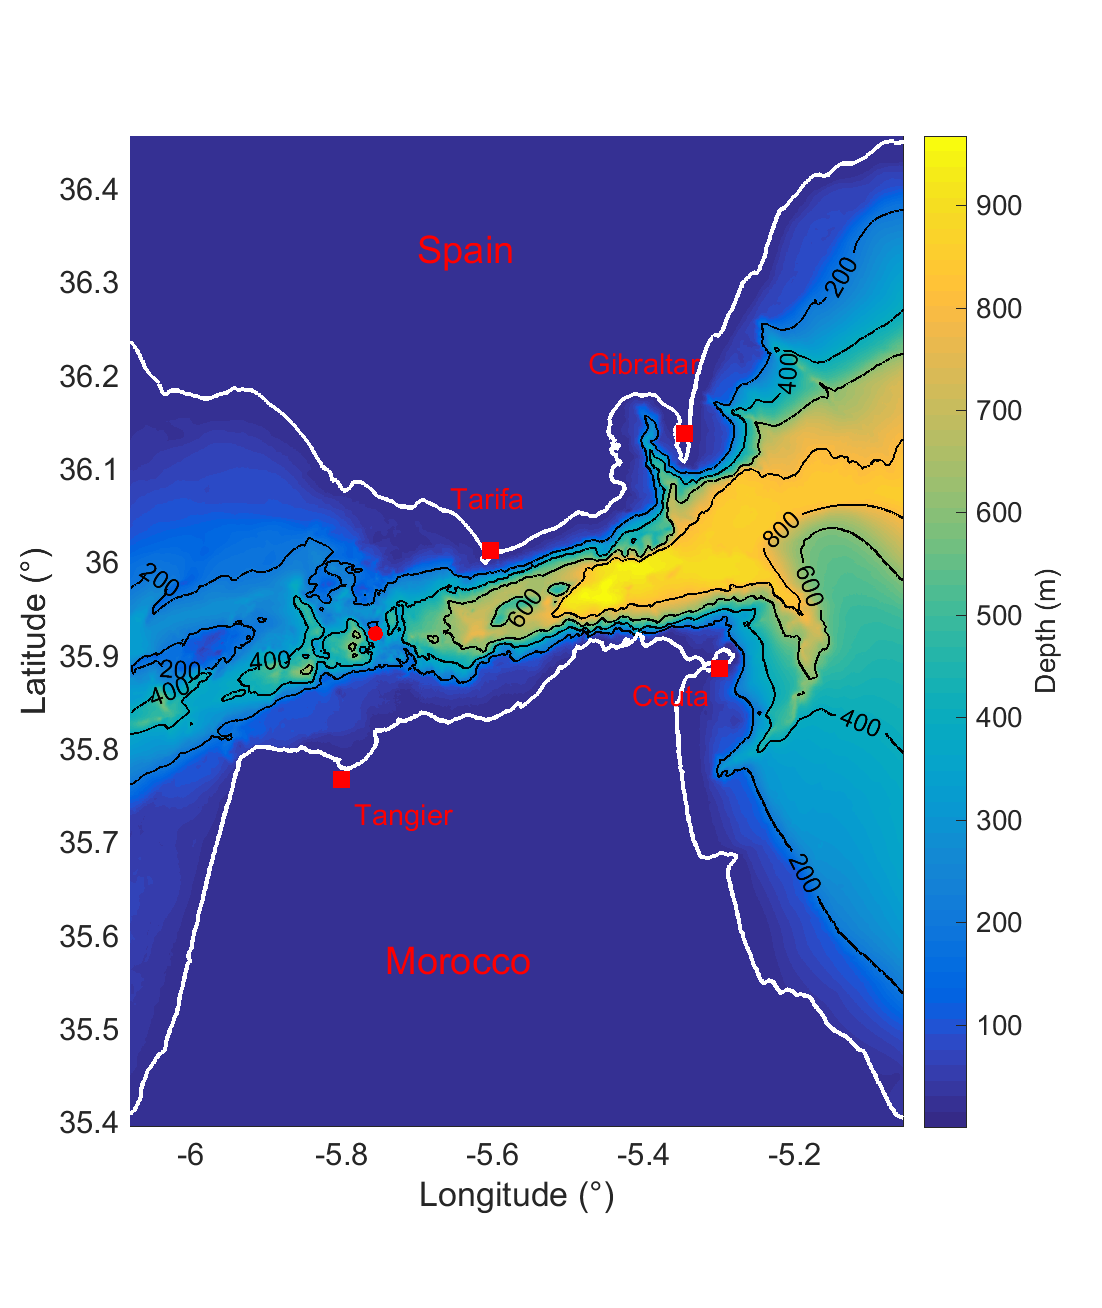
\includegraphics[width=0.5\textwidth]{./GBR3D/FigBathyVHR.png}
        \caption{Area and Bathymetry used for the simulations. The red dot denotes the point at Camarinal Sill where the zonal barotropic current is taken as reference in following figures.}
        \label{FigBathy3D}
\end{figure}



\begin{figure}[!h]
        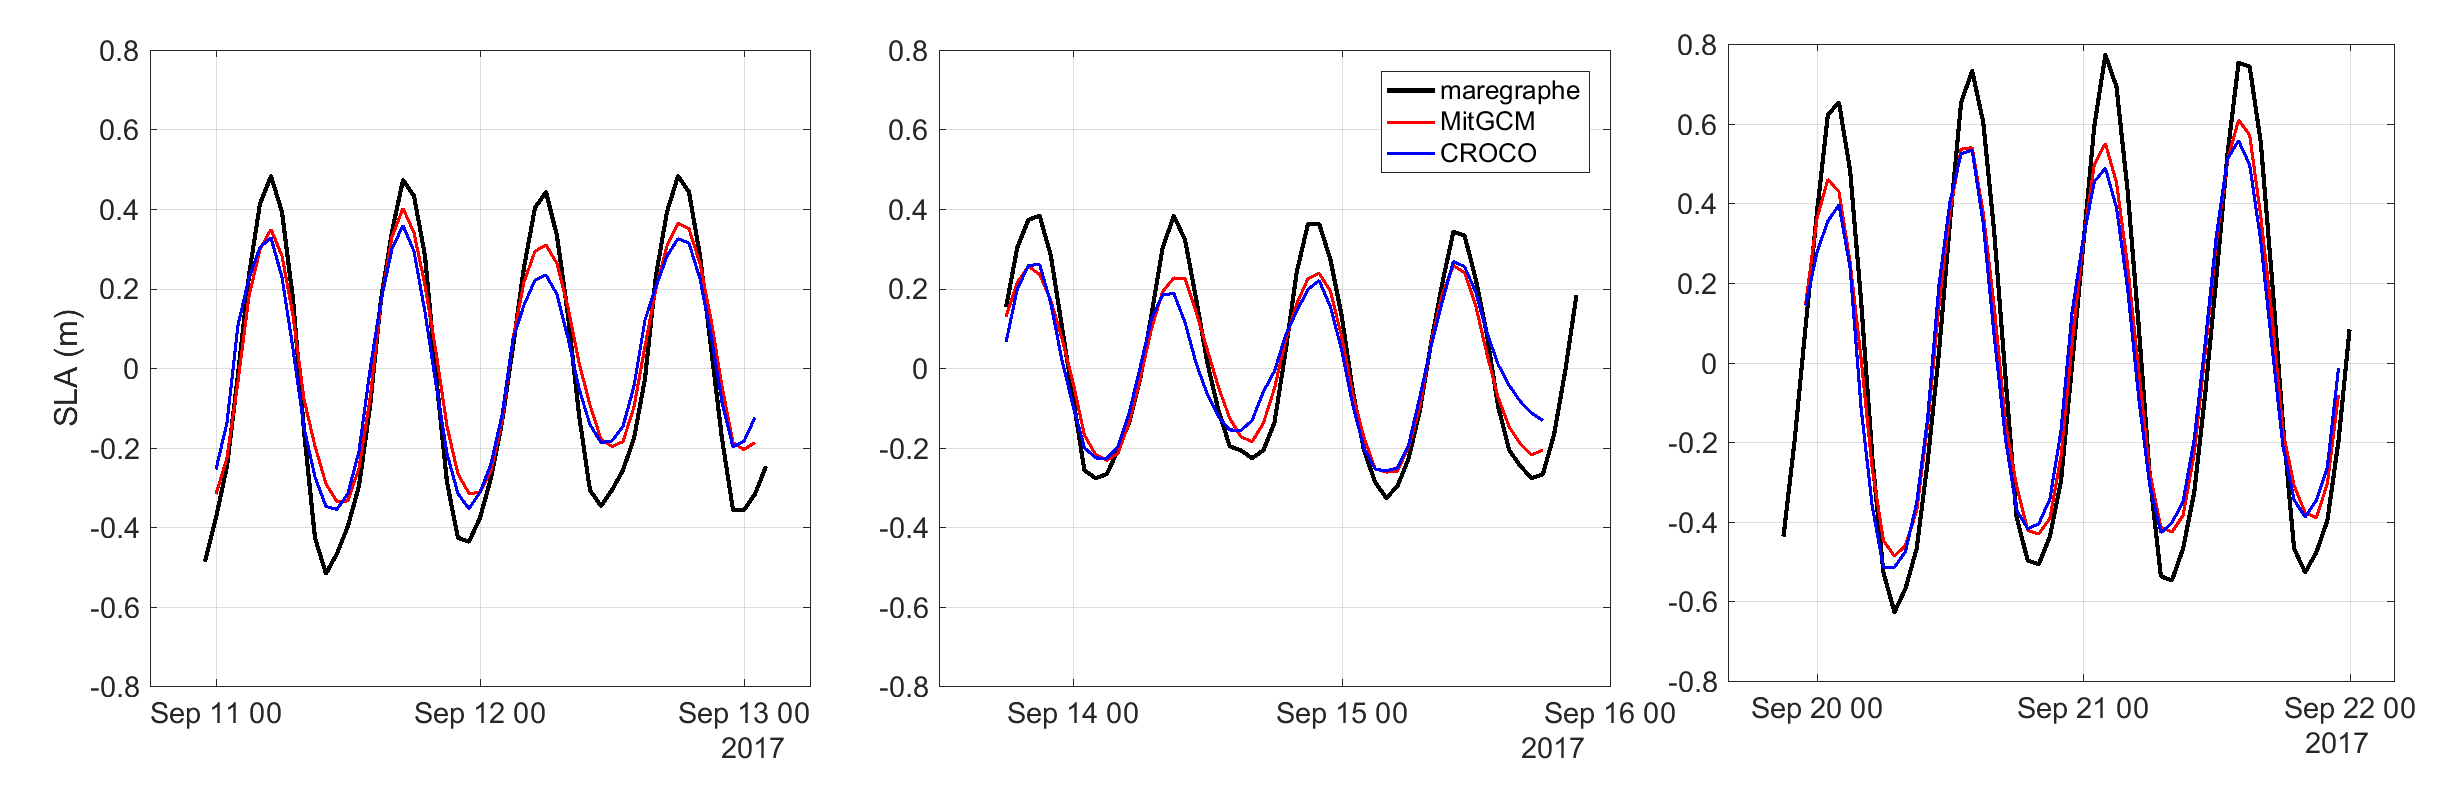
\includegraphics[width=\textwidth]{./GBR3D/SLA_Tarifa_ME2VE2IES.png}
        \caption{Sea level-anomaly at Tarifa from tidal gauge data (black) or at the nearest grid point for parent simulation (red) and CROCO simulation (blue), for situation ME (a), MM (b) et VE (c)}
        \label{fig_maree_tar}
\end{figure}

\subsubsection{Water masses}


\begin{figure}[!h]
        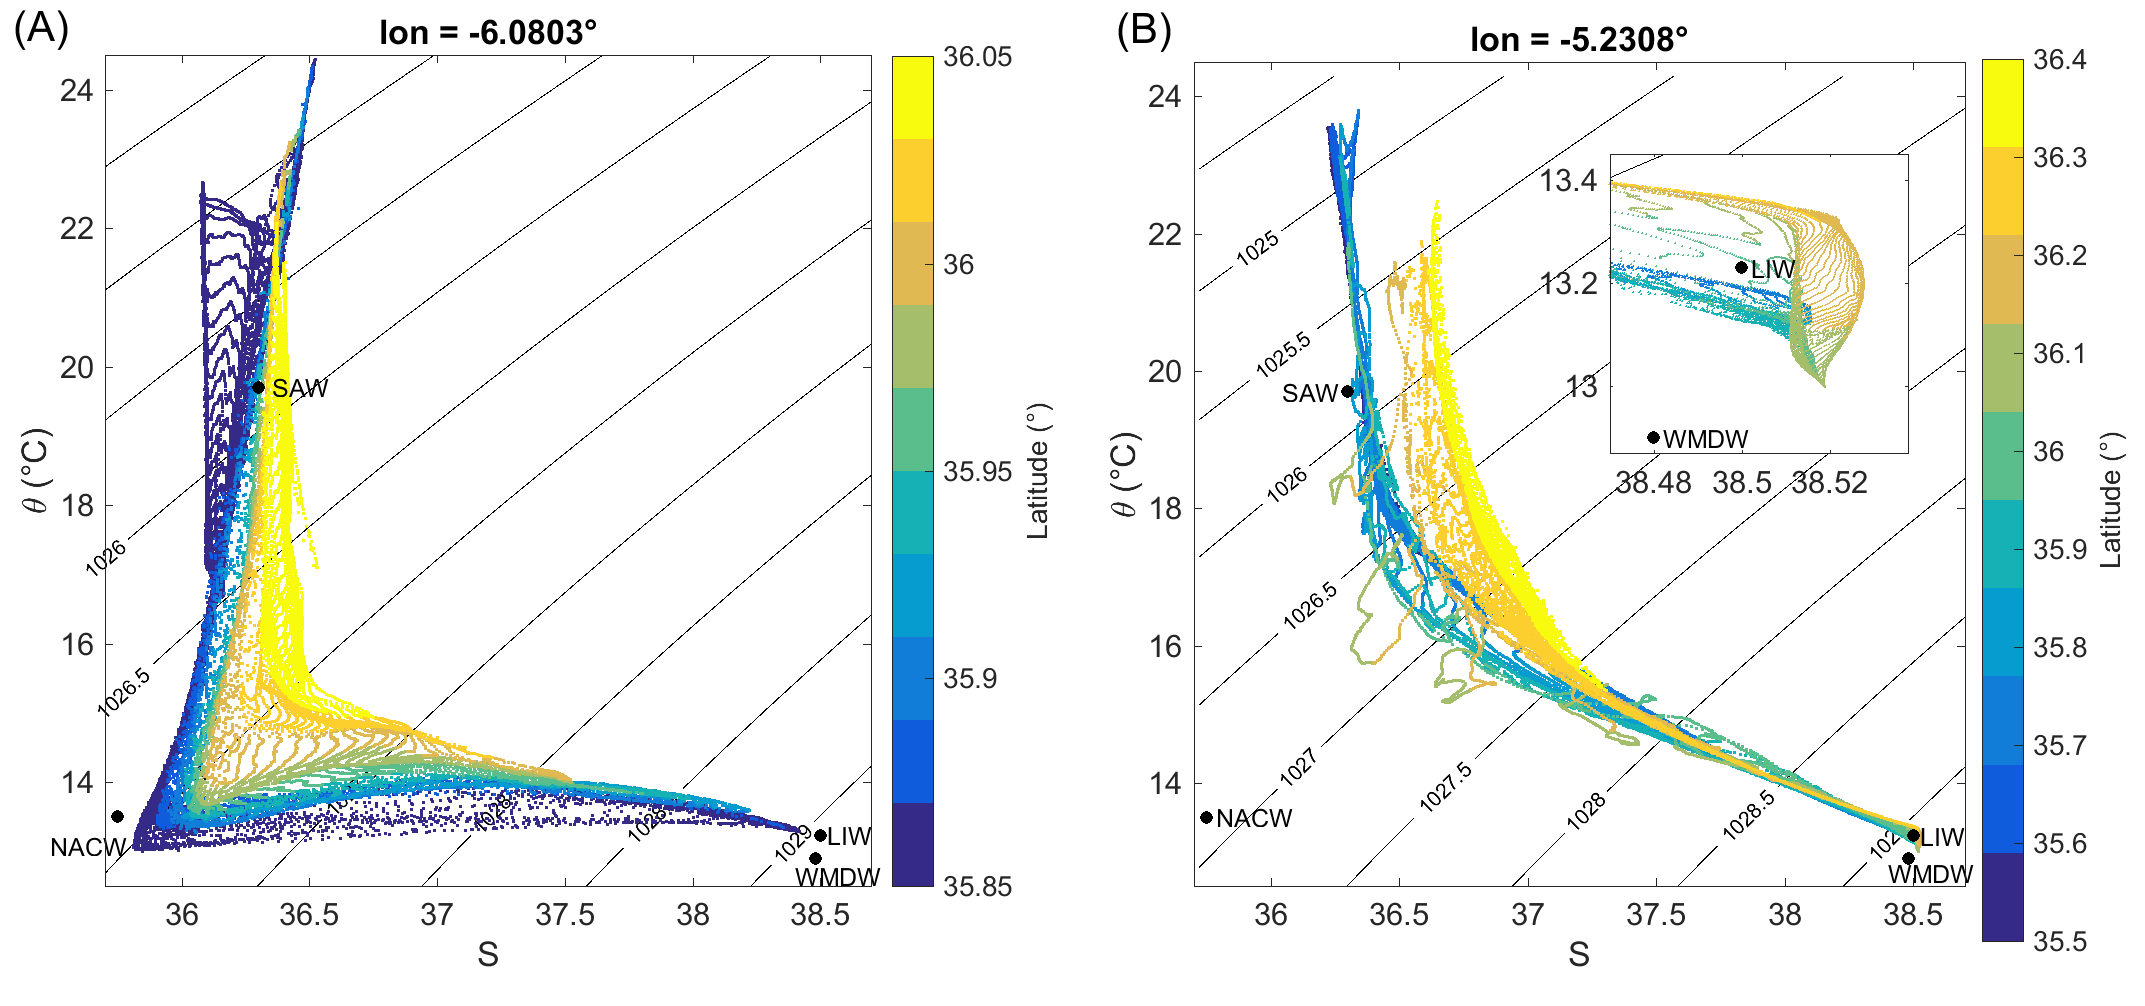
\includegraphics[width=\textwidth]{./GBR3D/WM_ini_IES.png}
        \label{Fig_Ini_WM3D}
\end{figure}


Figure \ref{Fig_Ini_WM3D} shows the $\theta$-S diagrams for east and west entry of the Strait in initial tracer field of simulation Intermediate Tide. As expected, for med waters see on the west side two signals for the two pathways of the med outflow, on the east side see distinctly a deep water mass and an intermediate one (not the value found in biblio) that could be interpreted as WMDW and LIW, with the latter being present mostly on the northern part, difficult to say if other water masses. For atl waters, NACW present on west of domain, less on east. On east, see difference surface water north/south.




\subsection{Numerical diagnosis}


\subsubsection{Interface definition}

The analysis of simulation result is based on two layer definition of an Atlantic waters layer and Mediterranean waters layer. They are defined in regard to a reference salinity, with the interface defined as the height of the first water parcel from the top down in teh water column for which salinity is above the reference salinity.

The reference salinity is taken as varying along the Strait as a hyperbolic tangente function of longitude centered at the Camarinal Sill to account for the different water mass composition in the eastern and western part of the Strait of Gibraltar. %The function was fitted against the median salinity found by of fitted hyperbolic tangente to the salinity profile in the water column for the initial field

%Take a two-layer approach to the dynamic and definition of atl and med layer.

%Following (Sannino?), the central salinity value of the interface is taken as the middle of the slope area in a hyperbolic tangent fit of the salinity profile at one grid point. This has been repeated for some ... accross the three simulations and along the Strait, can see that the pycnoncline is saltier east of the camarinal Sill. To define med and atlantic layer then chose a salinity of interface as a fuction of longitude :

\begin{equation}
	S_i(x)=tanh(\frac{x-X_{CS}}{DX})\frac{S_M-S_m}{2}+\frac{S_M+S_m}{2}
\end{equation}
with $X_{CS}=5.75^o$, $dx=0.25^o$, the location and width of the Camarinal Sill in degrees, $S_M=37.39$ and $S_m=37.1$ the max and minimum values taken respectively east and west of the sill.

%This may not give the perfect interface at any given time...

\subsubsection{Froude layer number}

With the atlantic and mediterranean layers defined as above, the Froude layer number for internal gravity wave is computed at each 2D grid point as : 

\begin{equation}
F_i=\frac{U_i^2}{g'h_i} , \ \text{with} g'=g \frac{\rho_2-\rho_1}{\rho_0}
\end{equation}

where $\rho_i$ averaged density in layer i,  $U$ is averaged velocity norm over the layer i of height h. If $F_i>1$ say that the flow in layer i is supercritical.


\subsubsection{Hydraulic Jump detection, acceleration of flow}

\begin{figure}[!h]
 \centering
 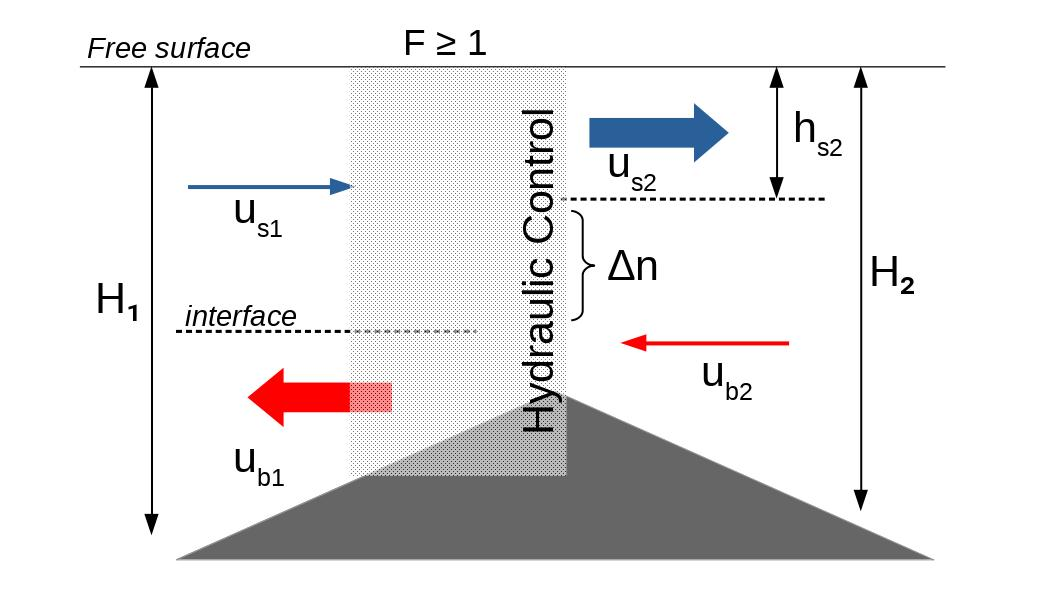
\includegraphics[width=0.5\textwidth]{./GBR3D/schema_diagressaut.jpg}
 \caption {Schematic of flow upstrean and downstream of hydraulic jump at Camarinal Sill, Strait of Gibraltar}
  \label{schemaRH}
\end{figure}


A simple diagnosis for detection of the hydraulic jump at Camarinal Sill in the simulations is based on the impact such a structure has on the flow. As schemtized(?) in figure \ref{schemaRH}, hydraulic jump (also called hydraulic drop) induces a drop of the interface depth. Since the flow in the Strait is cannalised by bathymetry (for med flow) and coast (for atl flow), there must be conservation of flux from one section downflow and upflow of the hydraulic jump, which with the variation of the inteface depth, means acceleration/deceleration of flow (depending on which layer is reference).

The drop in interface depth is noted $\Delta n=b_2-b_1$, the variation of bottom depth $\Delta H=H_2-H_1$ and the acceleration in the bottom layer $\Delta u_b = u_2-u_1$. For the bottom layer conservation of flux is :
\begin{subequations}
\begin{alignat}{2}
  \displaystyle
&u_1 (H_1-b_1)&& = u_2 (H_2-b_2)\\
& &&= u_1 (\Delta H + \Delta n) + u_1 (H_1-b_1) + \Delta u_b (H_2-b_2)
\end{alignat}
\end{subequations}

\begin{equation}
\Delta u_b = -u_1 \frac{\Delta H + \Delta n}{H_2-b_2}
\end{equation}

For the surface flow, similarly can find
\begin{equation}
\Delta u_s = -\Delta n \frac{u_1}{b_2}
\end{equation}

Velocity in the area of the hydraulic jump must validate condition of (at least) critical flow, ie Froude number $\geq$ 1. We search minimal condition for hydraulic jump so $F=1$ or $U=c$ flow equal propagation/phase speed of internal wave, if we take the interfacial speed can have an expression for $u_1$: 
\begin{equation}
|u_1|=c=\sqrt{g' \frac{(H_1-\Delta n - b_2)(\Delta n + b_2)}{H_1}}
\end{equation}



In the end, some parameters are chosen as threshold, here take values that should be correct for area of camarinal sill, the minimum excursion of the jump $\Delta n = 30m$ and the height of the Atl layer $b_2=50 m$ , and the reduced gravity $g'=0.02 m s^{-2}$.

\subsubsection{Q parameter and derivated diagnosis}

We want to detect primary shear instabilities in the Med outflow. A simple vorticity diagnosis is not chosen because it requires chosing the rotation axe and regions of high shear such as between the MEd outflow and Atl waters, have high vorticity values. Insetad, chose to compute parameter Q, as defined as :

\begin{equation}
Q=-\frac{1}{2} \frac{\partial u_i}{\partial x_j} \frac{\partial u_j}{\partial x_i} = \frac{1}{2} (\Omega_{ij}\Omega_{ij} - S_{ij} S_{ij})
\end{equation}
with $u_i$ the component of velocity, and $S_{ij}$ and $\Omega_{ij}$ are respectively symetrical and anti-symetrical parts of velocity gradient (comme ça se dit en anglais????). When $Q>0$, anti-symetrical term contribution, which denotes rotation, is predominent over the symmetrical, shear, part. ((It can also be viewed as a generalisation of Okubo-Weiss parameter used in 2D, however rotation is indicated by negative values for OW, but by positive values for Q parameter.))

%This distinction between shear an rotation is not achieved by a simple vorticity calculation // Also $Q>0$ better to detect vortices than just vorticity since there is still then shear between med vein and atl layer.


Due to advection by the Med outflow, a succession of primary instabilities will propagate over teh same grid cells. The temporal evolution of Q over such grid cell will show oscillations between high positive value (center of a billow/vortex) and low negative values (shear between two consecutive billows). A proxy to detect this area is chosen as high value of standard deviation of parameter Q, as defined in equation \ref{eqstdQ} where the overbar denotes temporal average over 30 minutes, a period over which there will be minimal modification of the general flow in the Strait.

\begin{equation} 
\label{eqstdQ} 
    std ( Q ) (\vec{x},t)=  \sqrt{   \overline{Q (\vec{x},t)^{2}} -  \overline{Q(\vec{x},t)}^{2}  }
\end{equation}

To create 2D maps, only the maximal value of standard deviation in the water column is saved...
By implementing this calculation directly in the code, we can asses where instabilities/vortexes propagate without having to make a huge volume of simulation outputs over the whole domain, those economising in storage place and data readability. Thus it is possible to create a map of standard deviation of Q which will reflect areas where KH billows will propagate in the simulation.

The result of this proxy can be compared to the result of the Singular Value Decomposition (SVD) of the time-varying 3D field. However thhis calculation is offline and necessitates a high frequency 3D output to pick up the relevent structures.



\subsection{Results}


\subsubsection{Flow criticality/Hydraulically controlled layer and hydraulic jump, neap-spring tide variability}

ATTENTION courant de gravité et ressaut hydraulique...


\begin{figure}[!h]
 \centering
 
 \begin{subfigure}{\linewidth}
\centering
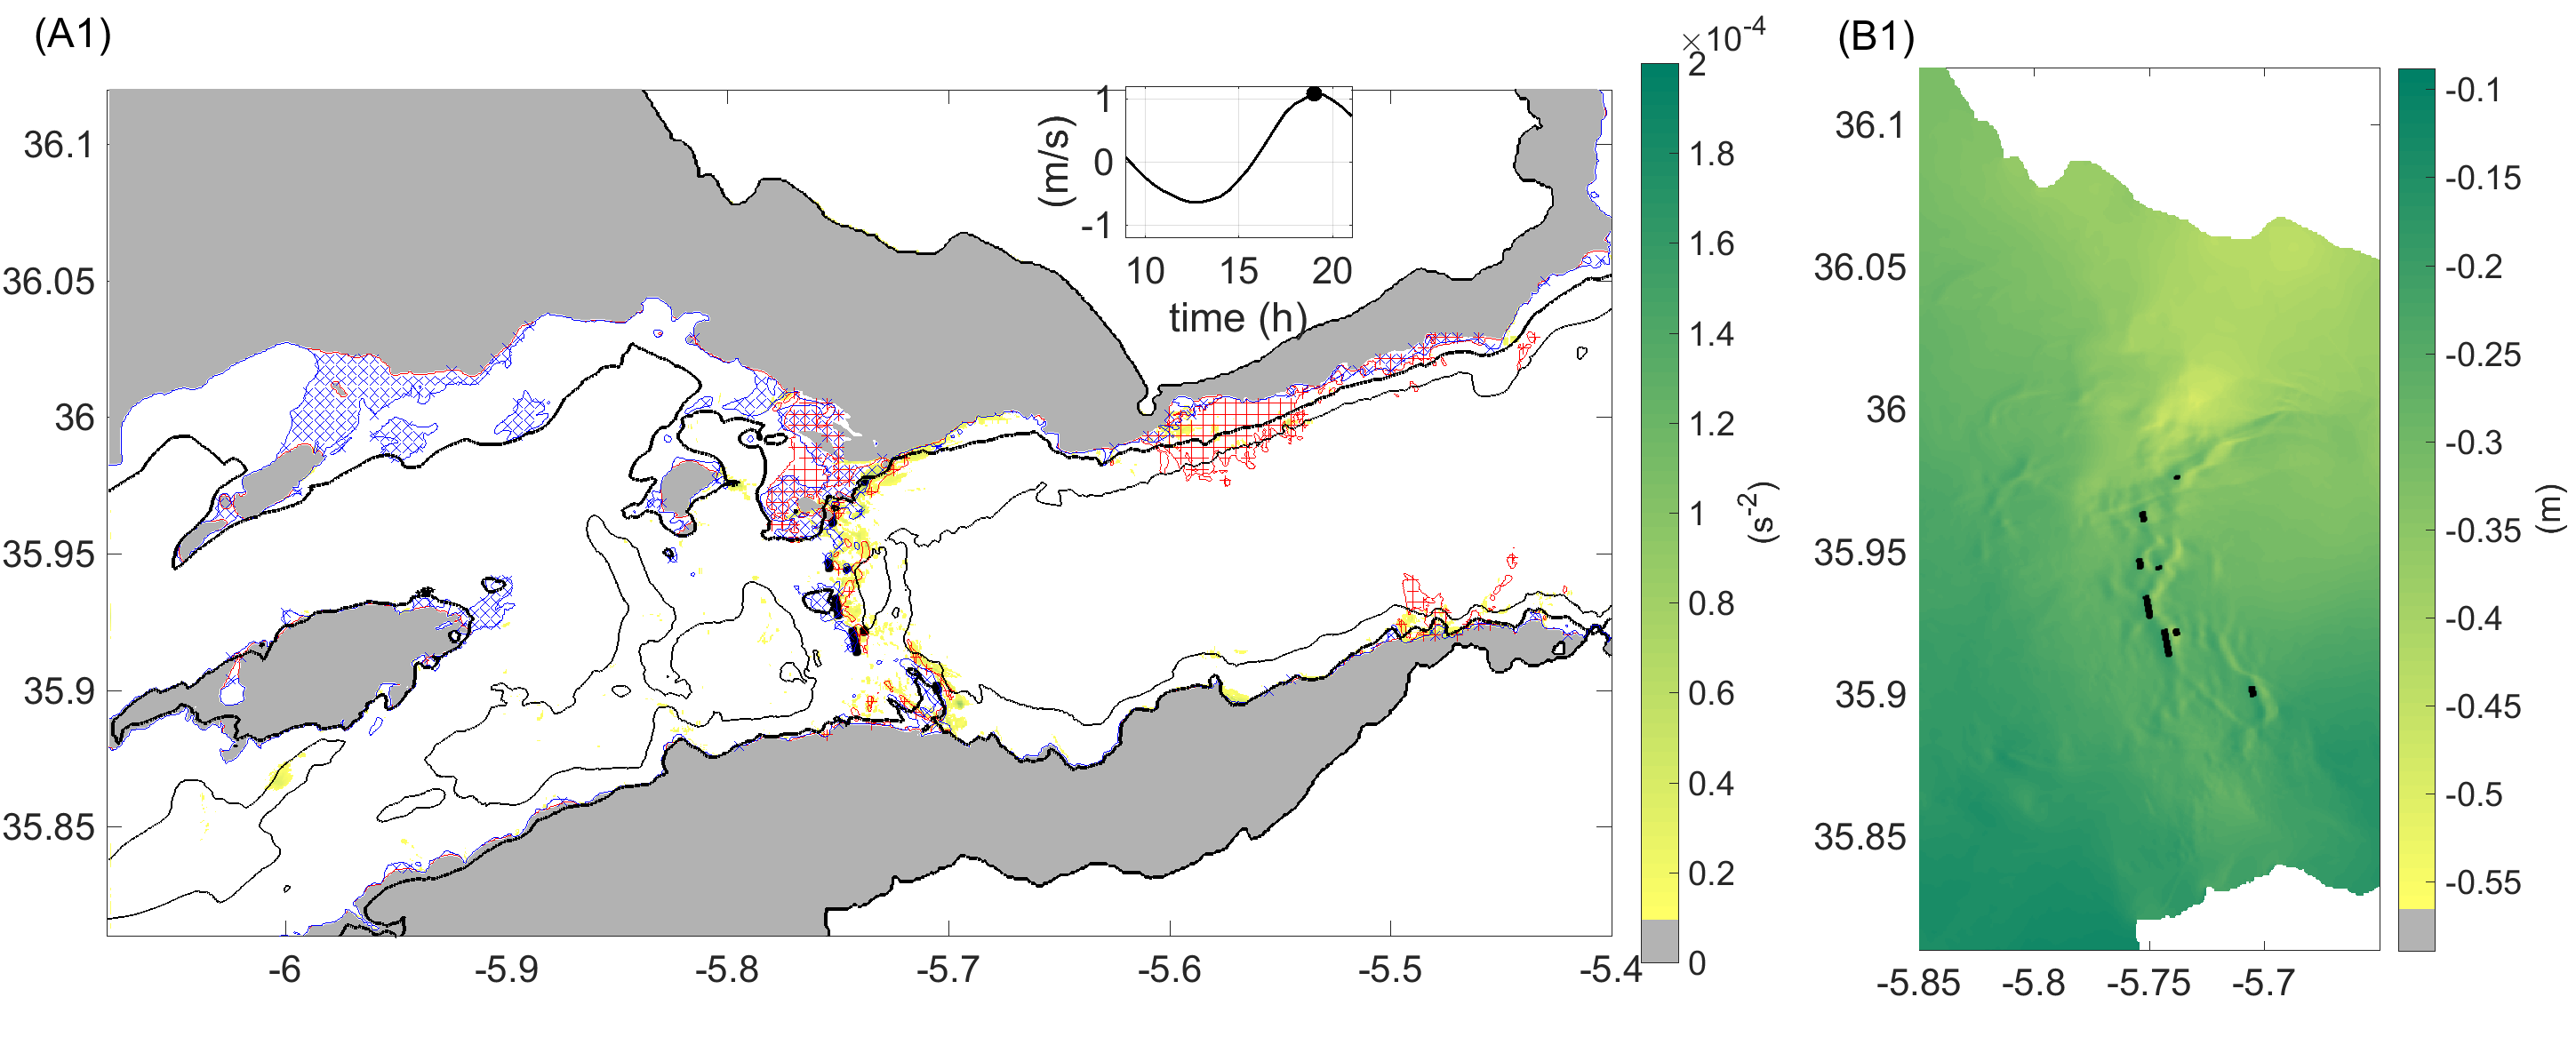
\includegraphics[width=1\linewidth]{./GBR3D/ME2_19h_p.png}
\end{subfigure}
 
 \begin{subfigure}{\linewidth}
\centering
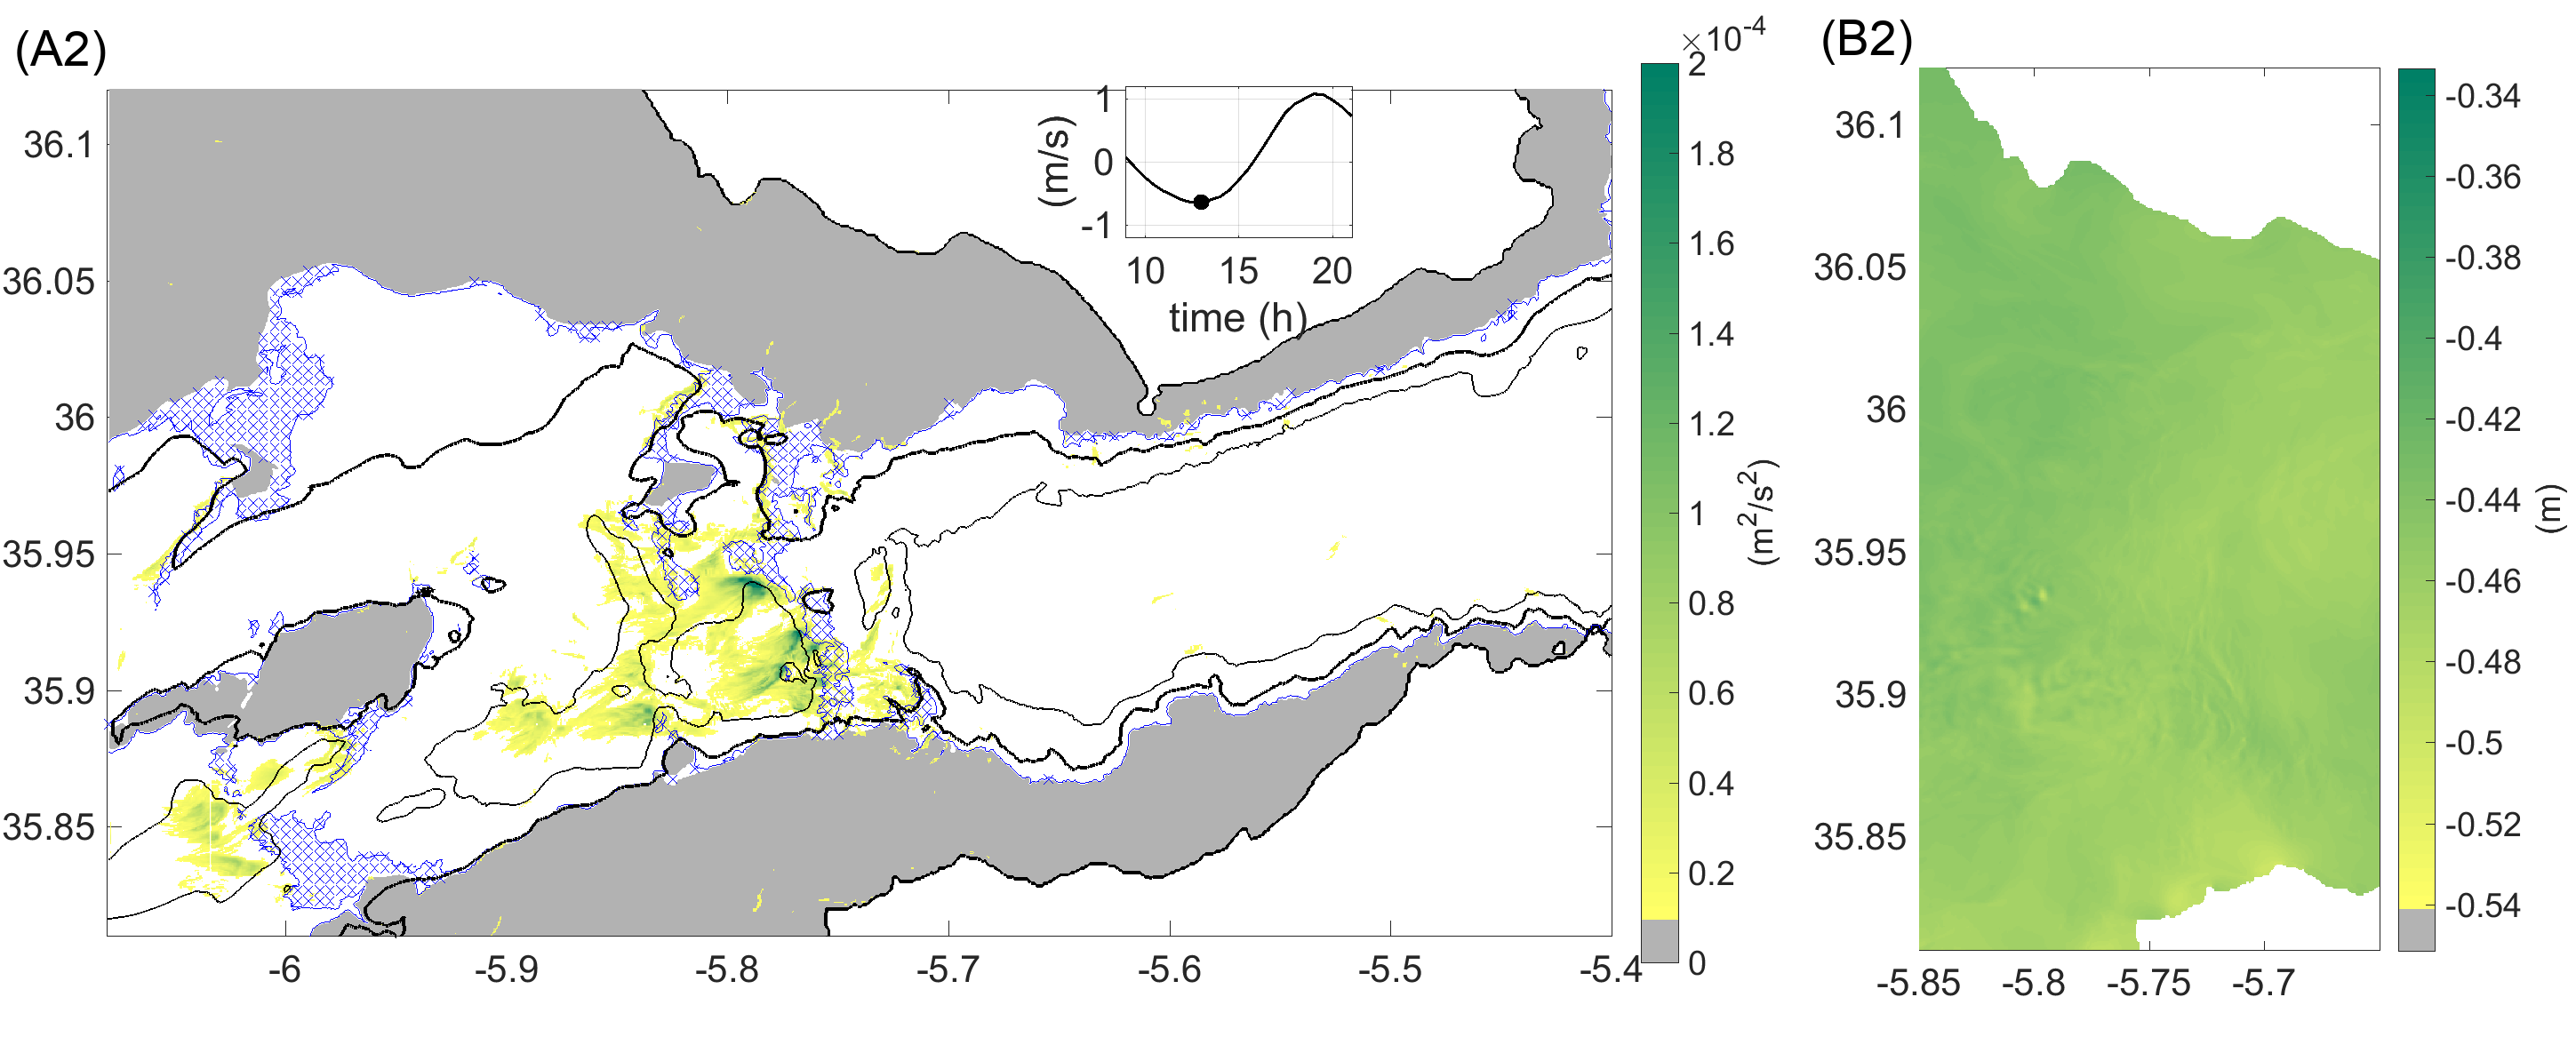
\includegraphics[width=\linewidth]{./GBR3D/ME2_13h_p.png}
\end{subfigure}
\caption {For simulation SimNT, an inflow then an outflow of type \textit{no-jump}. Blue (red) shaded area is supercritical med (atl) layer. Black dots are hyd jump detection. grey area denotes where S bottom$<$Sinterface. colorbar for standard deviation of parameter Q (only values above $10^-5$are represented). Also inicated barotropic znal current at 5.7553$^o$W  35.9238$^o$N. Two black isobathes contours are indicated, 200m (bold) and 400m(thin) depth  }
\label{FigHCN}
\end{figure}

Figures \ref{FigHCN} to \ref{FigHCI} present several diagnosis for series of maximal outflows and inflows for variable strength of the tidal forcing among simulations NT,ST then IT. Are represented the area of supercritical flow in atl and med layer as defined in paragraph .., the detection of hydraulic jump as per paragraph ..., and area of standard deviation of parameter Q, which indicate were vortices are propagating. The grey area indicates where the salinity in the bottom level was below the interfacial salinity as defined in paragraph ... .

Figure \ref{FigHCN} presents weak barotropic tidal currents in outflow and inflow and is considered a 'neap-tide' case, figure \ref{FigHCS} is for strong brotropic currents for the in- and outflow of a 'spring-tide' case. Finally, figure \ref{FigHCI} is the case of an outflow for an intermediate strength of the barotropic currents.

\begin{figure}[!h]
 \centering
\begin{subfigure}{\linewidth}
\centering
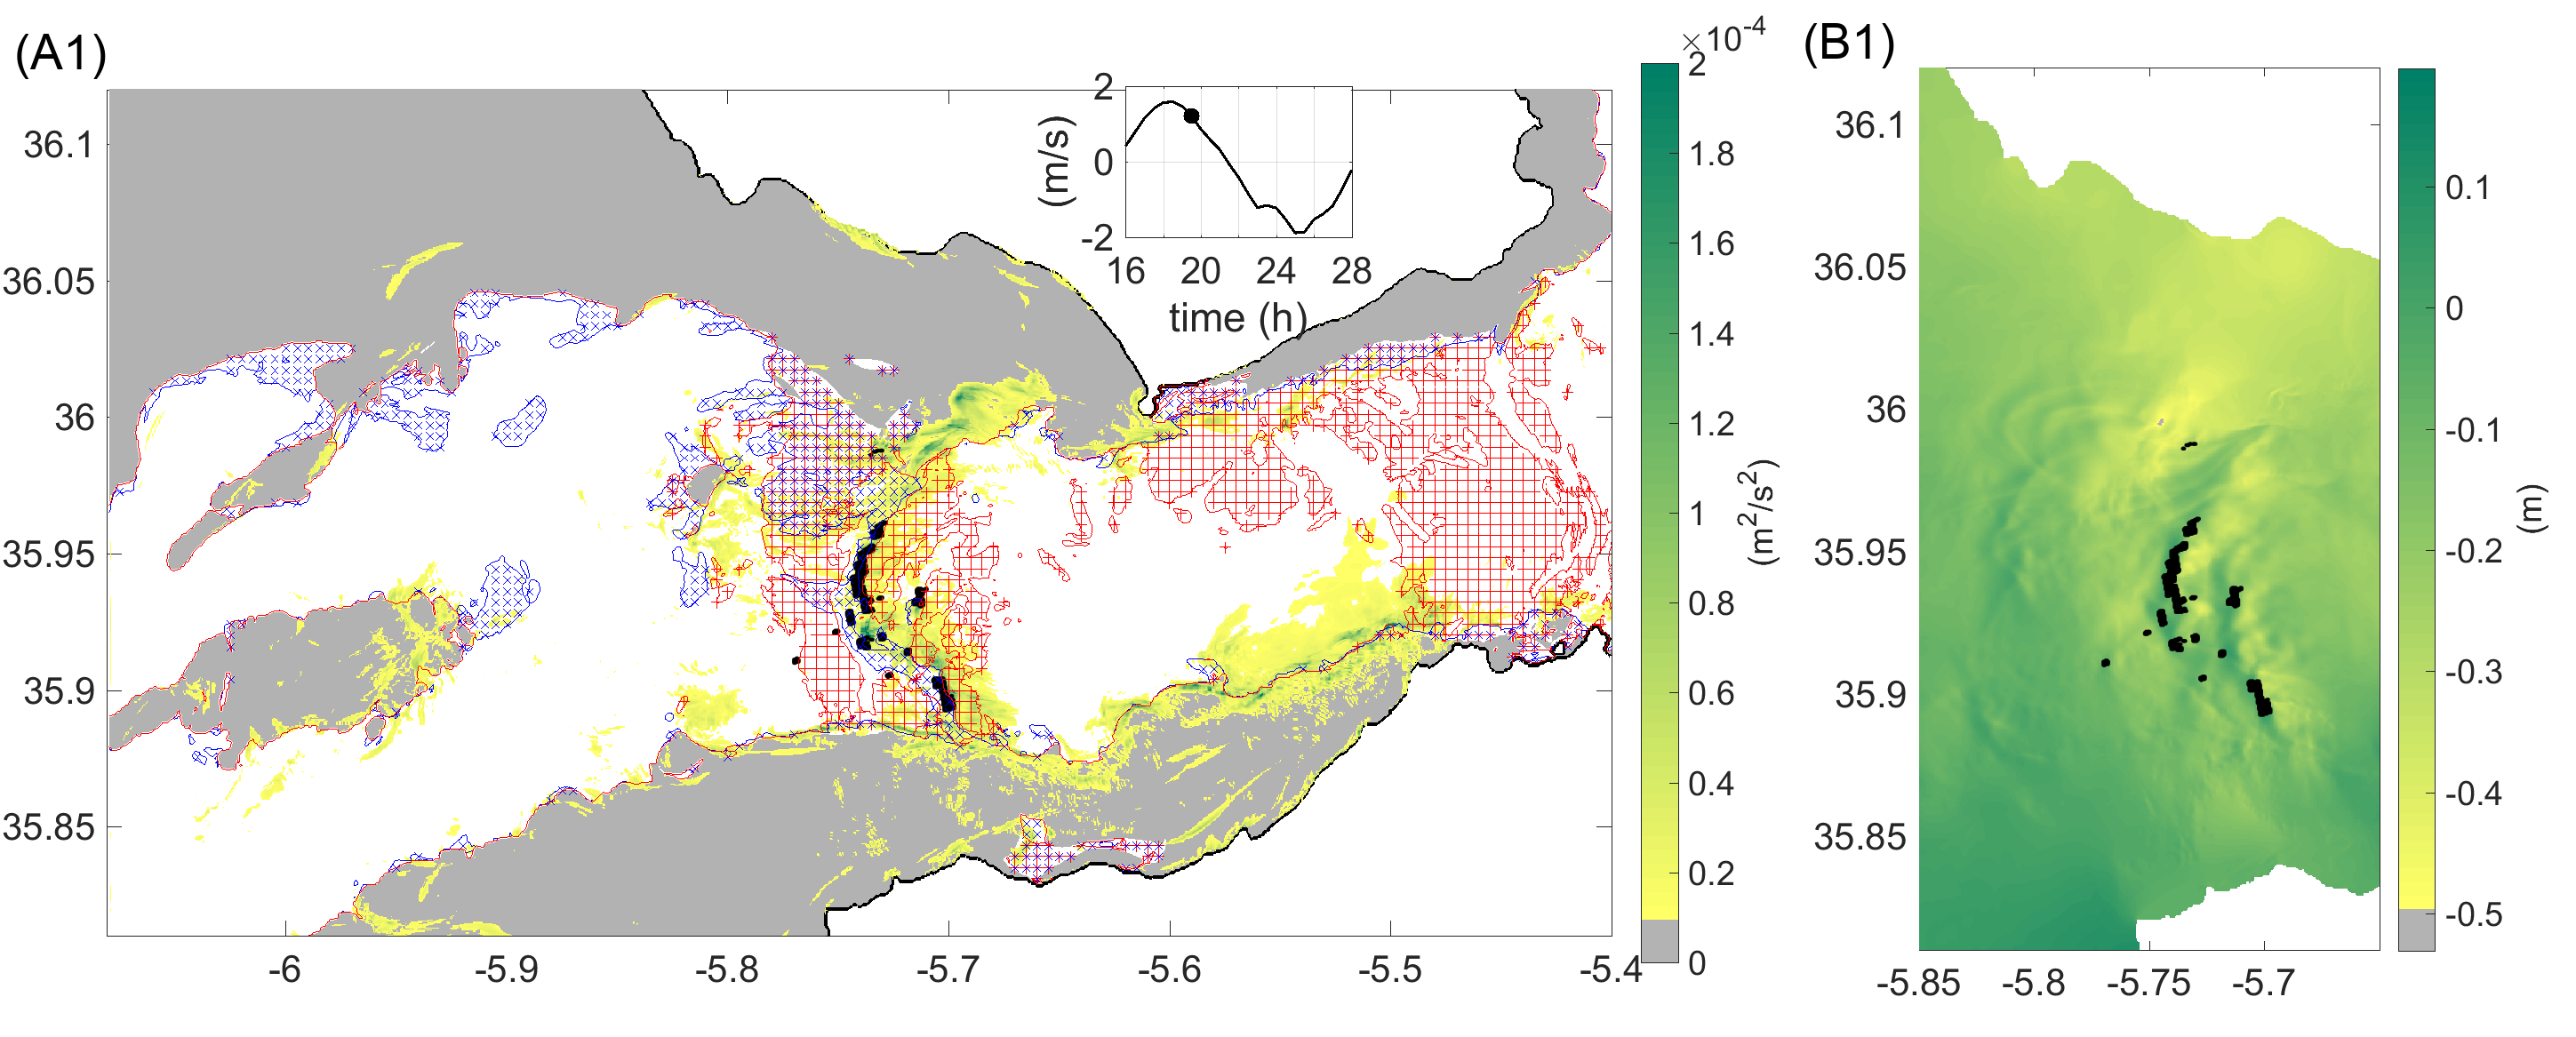
\includegraphics[width=\linewidth]{./GBR3D/VE2_19h30_p.png}
\end{subfigure}

\begin{subfigure}{\linewidth}
\centering
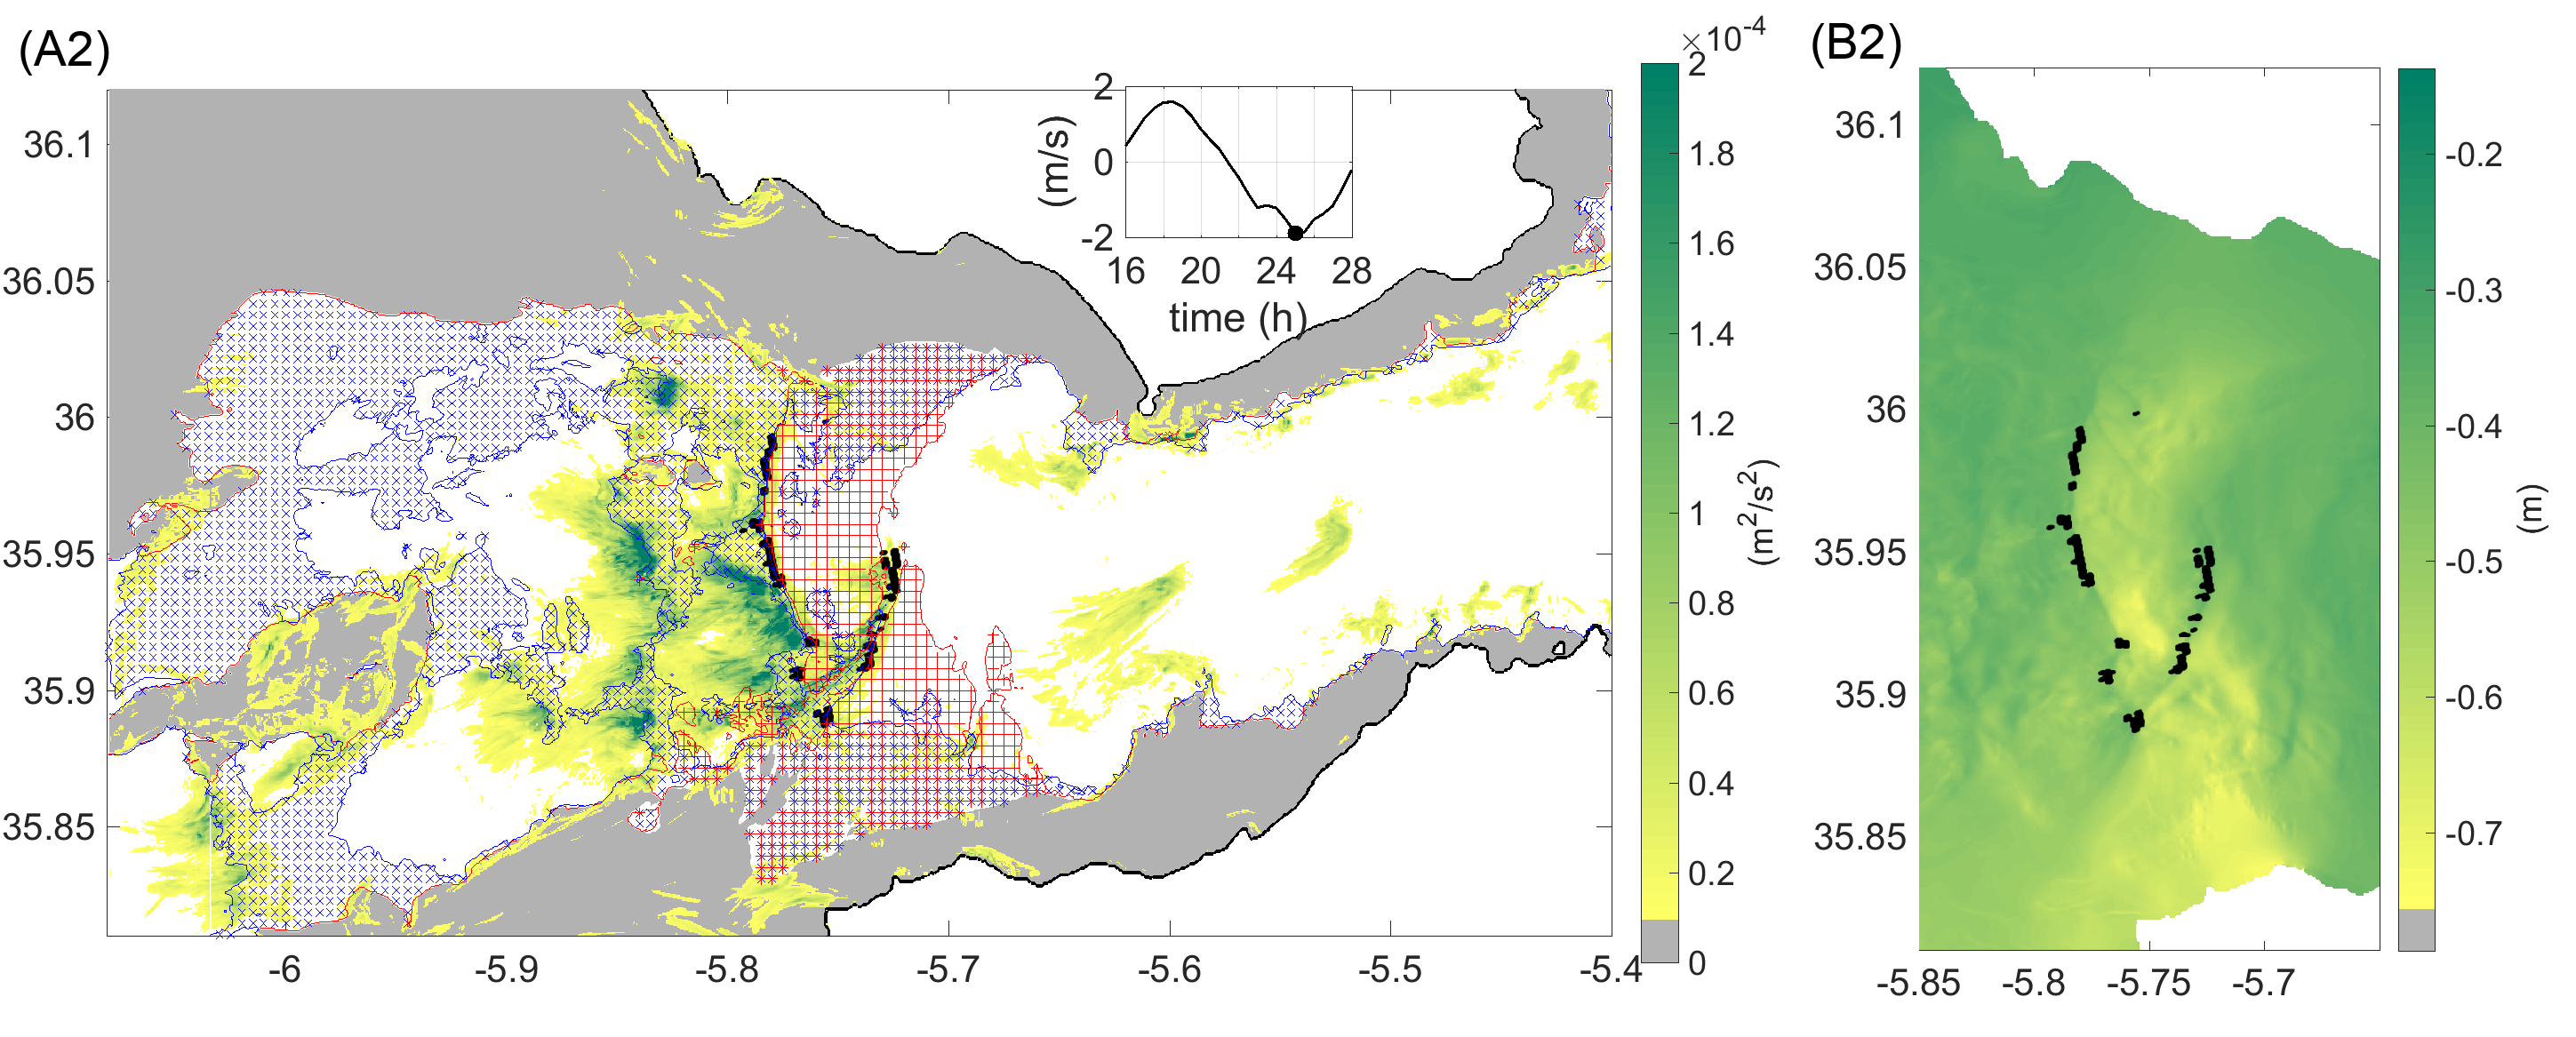
\includegraphics[width=\linewidth]{./GBR3D/VE2_25h_p.png}
\end{subfigure}
\caption {Same as figure \ref{FigHCN} for simulation SimST in inflow and outflow of type \textit{w-jump}}
\label{FigHCS}
\end{figure}

\begin{figure}[!h]
 \centering
%\begin{subfigure}{\linewidth}
%\centering
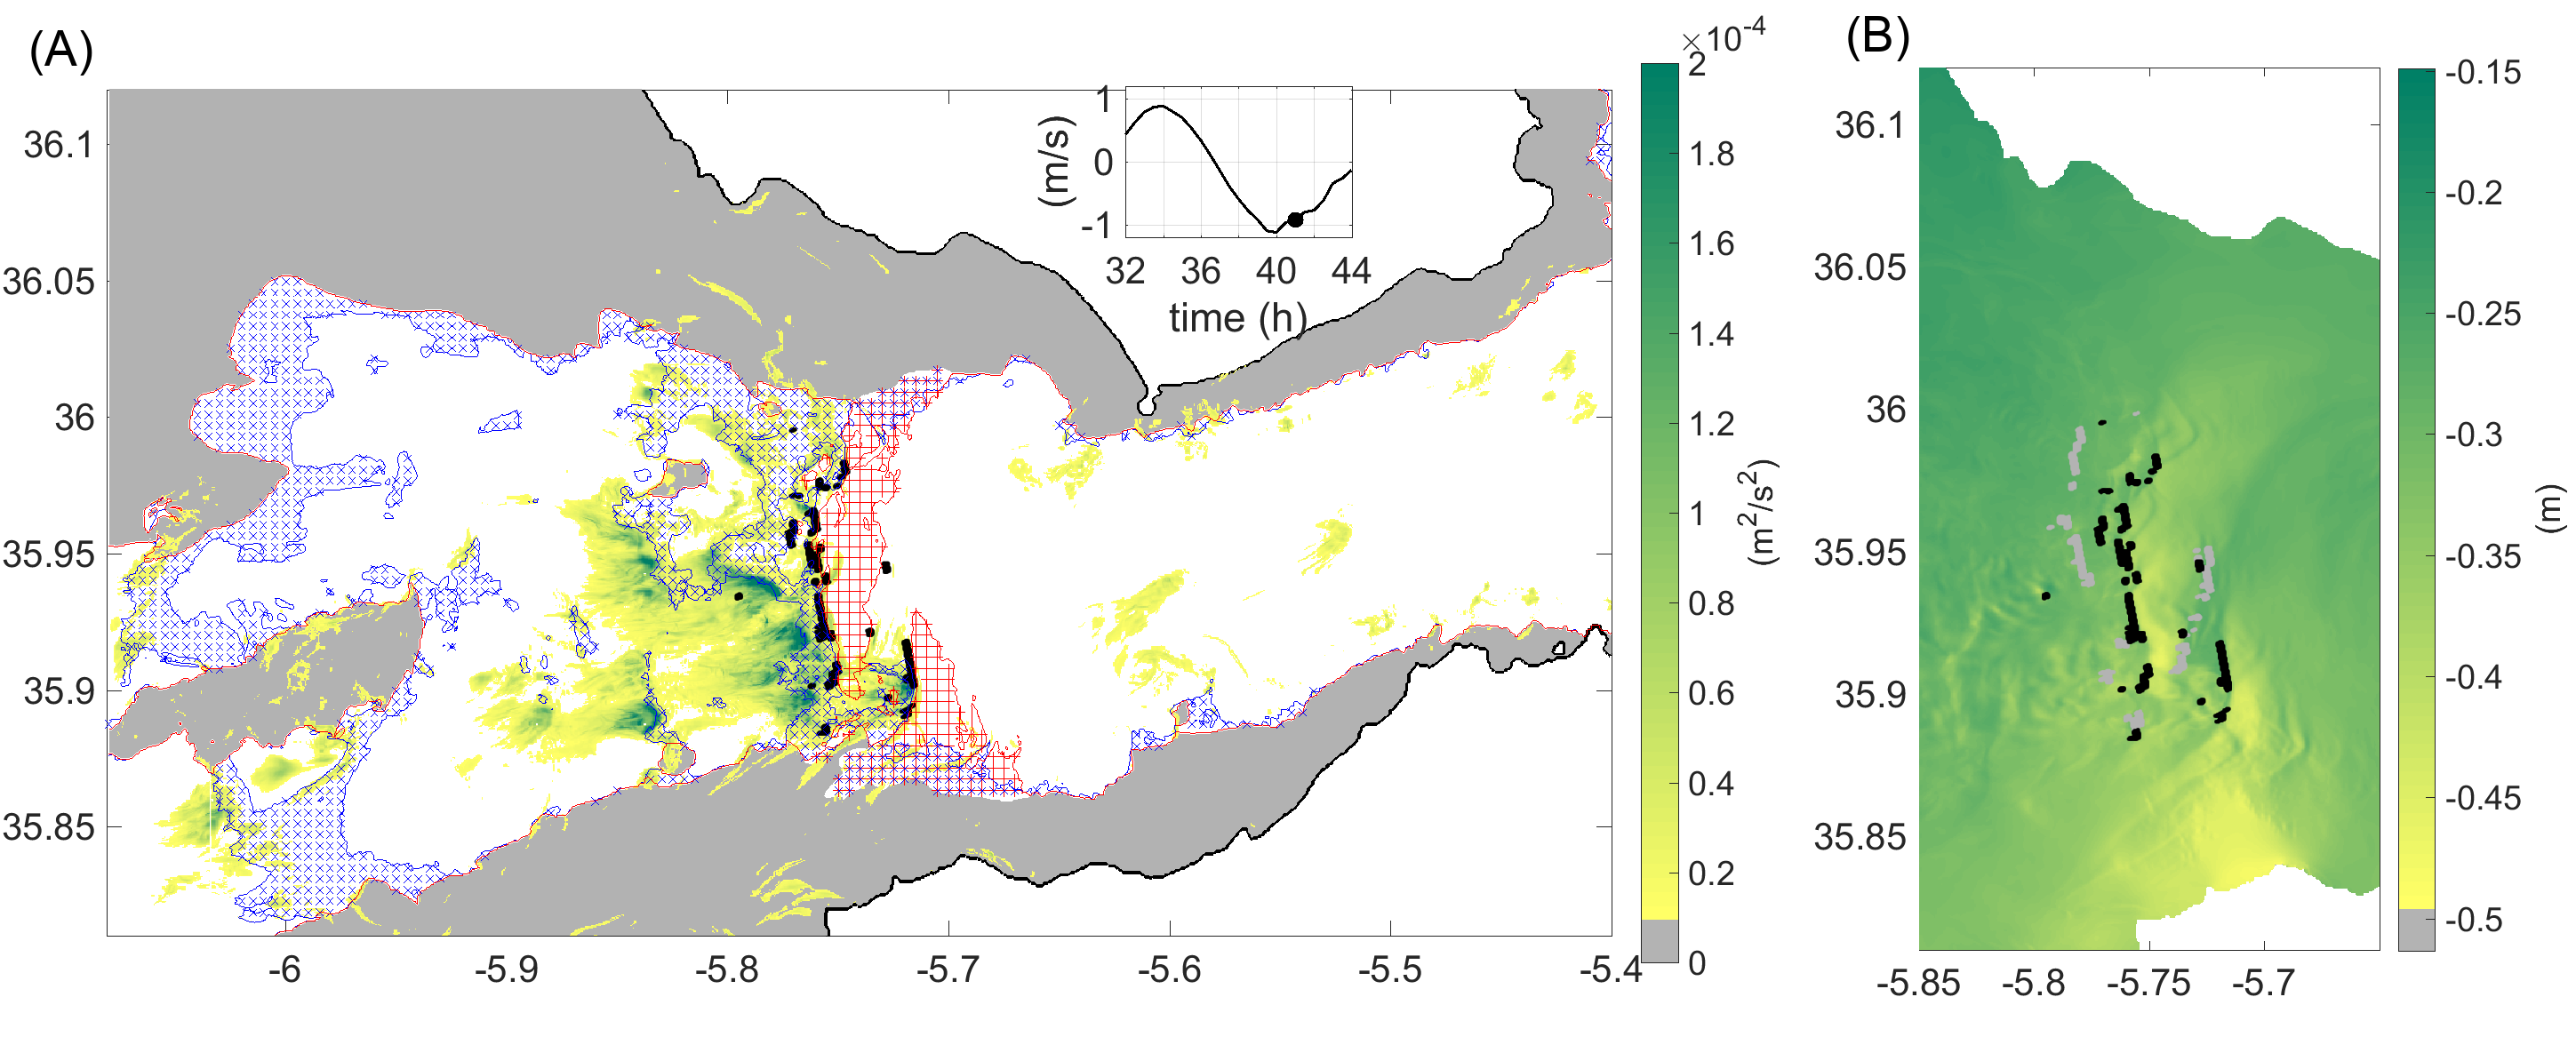
\includegraphics[width=\linewidth]{./GBR3D/IES_41h_p.png}
%\end{subfigure}
 \caption {Same as figure  \ref{FigHCN} for simulation SimIT and an outflow of type {s-jump}, on figure SLA also put trace of jump of spring tide outflow}
 \label{FigHCI}
\end{figure}

Firstly, can see two channels west of the Camarinal Sill where Med layer is present, separated by Majuan Bank. The path of the med vein through the south channel does not change much, however in the northern channel see a variable area of cicrulation for med waters above 200m depth and centered at 36$^o$ N. This area is larger while in outflows, as new med waters go upsolpe due to the westward barotropic current, but there is also a southern component to the flow that bends back into the main north channel (see figure (bathy) for a better view of the bathymetry of the area).

For all cases, supercriticality of the atlantic (mediterranean) layer happens mostly east (west) of 5.8$^o$W which is the western slope of Camarinal sill. During inflows in figure \ref{FigHCN}.a and \ref{FigHCS}.a, criticality of the mediterranean layer only occurs in patches, the most extended one in the area of the nothern channel discussed above. In outflows in figures \ref{FigHCN}.b,\ref{FigHCS}.b and \ref{FigHCI} the Mediterranean layer is supercritical at both Camarinal,Espartel Sill and nothern channel for all cases. In spring case outflow most of the nothern channel has a supercritical flow (descrip crit med layer outflow...)


During outflow suprcritical atl layer only at CS, except in neap case where it does not occur at all. in inflows, for neap case it is critical only at a patch near nrth shore in TN at 5.59$^o$W and north part of CS. for spring tide case, it is supercritical at TNboth as a more extended patch of the one of the neap case and a greater patch going north/south between 5.5$^o$W and 5.4$^o$W , and at CS. Figure \ref{FigISWGBR3D}(onde a TN) shows the fiel of surface current divergence in Tarifa Narrows while a train of ISW is propagating, igure a for condition of inetrmediate strength of barotropic current in inflow and figure b for a strong barotropic current at the same time as figure \ref{FigHCS}.b. Are also shown the areas of critical atlantic layer flow as black mesh area. The propagation of the ISW train occurs at the same time as maximum inflow in this area and sea the area of atl layer criticality is after . it seems the northern part of the criticlaity of the atl layer is dissociated from its southern part. The former is occurs often and is more or less extended while the other may be affected by influence of the passage of the ISW be it i the form of induced velocity or stratification.

Those propagating ISW are developped from hyd jump that are detected in figures... for all cases except the neap tide outflow. It is (usually) located at the junction between an area where atl and med layer are supercitical. It follows area of high gradient of free surface elevation. The shape of the hydraulic jump in inflow is more pronounced for stronger barotropic currents. For outflows, two different shapes are seen accross the simulations when hydraulic jump is formed, in spring tide at first resembles the intermediate case//at first the hyd jump forms at the top of the sill, but as the tidal barotropic current strenghten the hydraulic control on the atl layer expends west, but as barotropic currents increase jump is swept wesward as the area of supercritical atl layer extends over the sill.

Find accross all simulated tidal cycle three type of flow at Camarinal Sill during outflow : no hydraulic jump as in figure \ref{FigHCN}.b (\textit{no-jump}), a hydraulic jump situated just above the sill (figure \ref{FigHCI}, \textit{s-jump}), and a hydraulic jump situated over the west slope of the Camarinal Sill (figure \ref{FigHCS}.b, \textit{w-jump}).

\begin{figure}[!h]
 \centering
%\begin{subfigure}{\linewidth}
%\centering
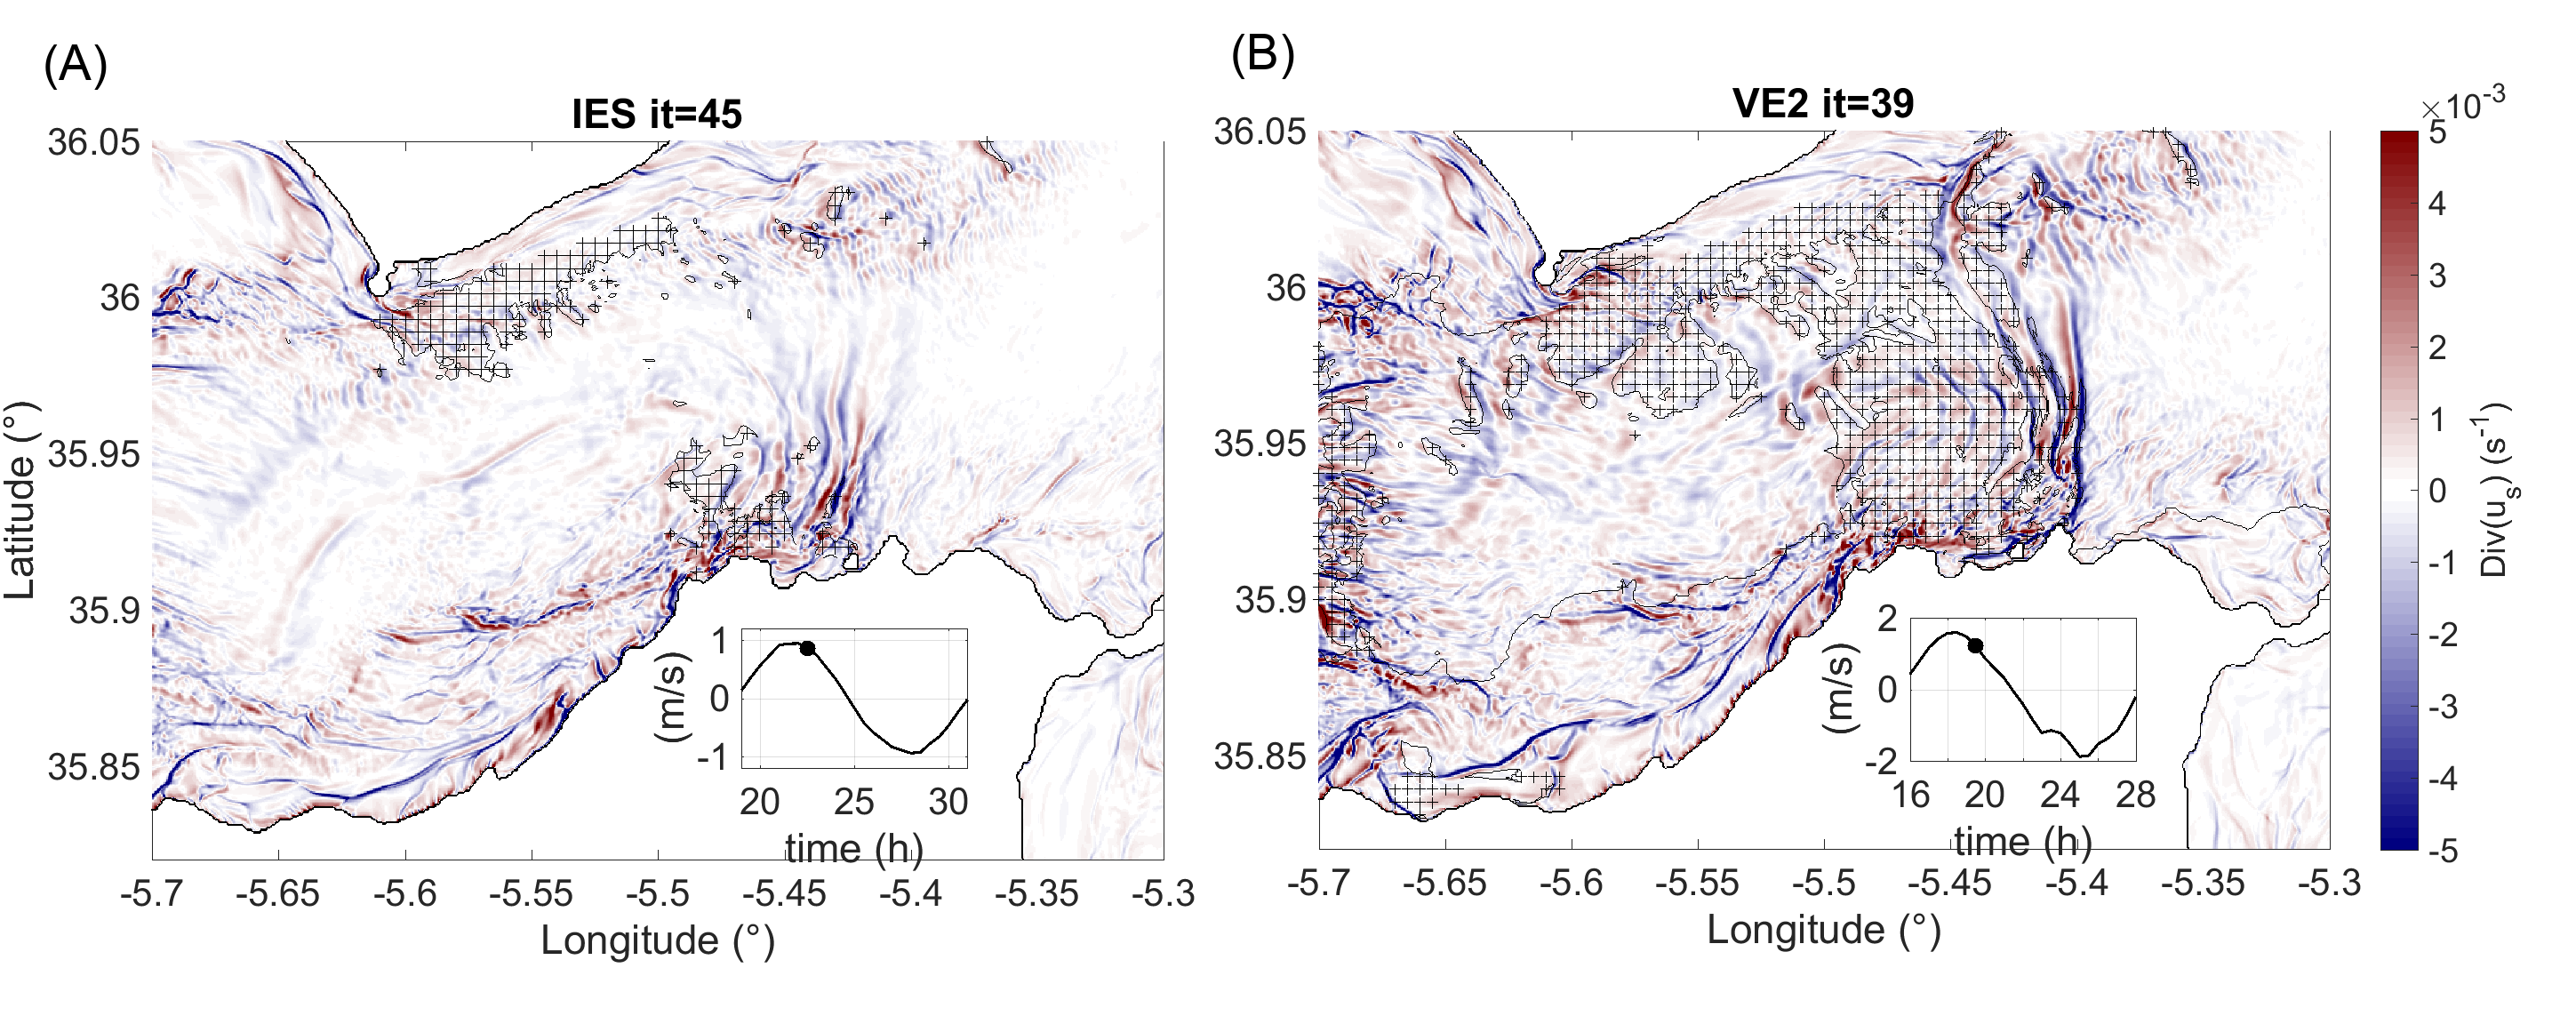
\includegraphics[width=\linewidth]{./GBR3D/FigWaveCont.png}
%\end{subfigure}
 \caption {Divergence of surface current (color) and area of supercritical atlantic layer (black hatchs) at t=22.5H in SimIT (a) and t=19.5H in SimST (b)}
 \label{FigISWGBR3D}
\end{figure}


\subsubsection{Propagation of Solitons (ISWs)}



\begin{figure}[!h]
 \centering
 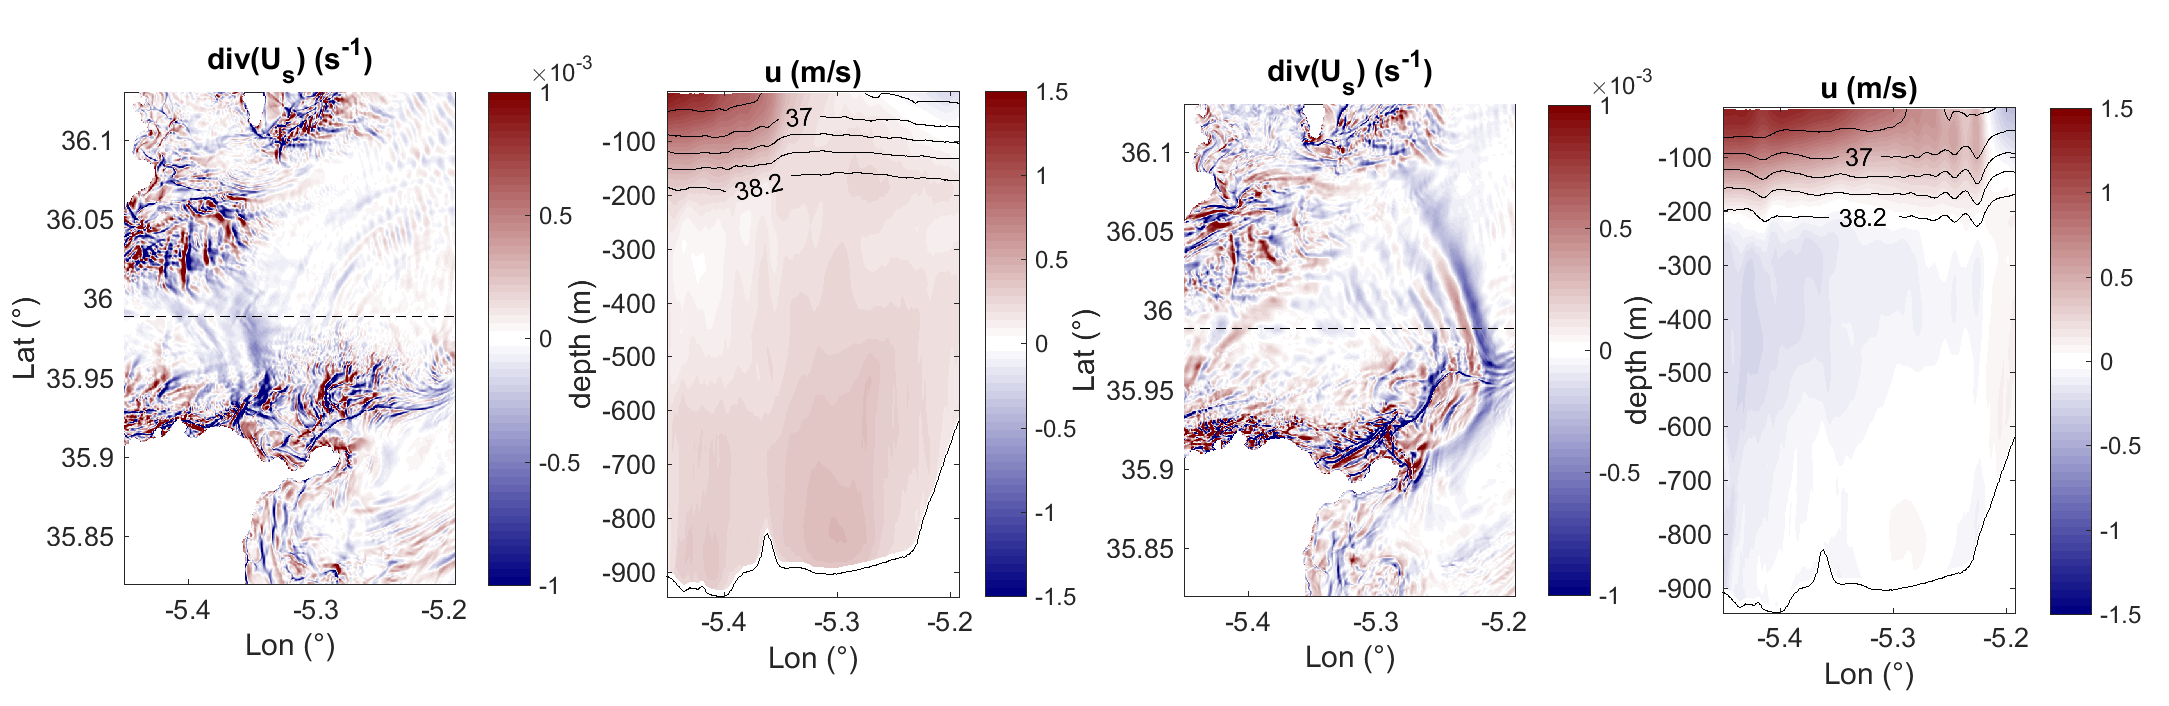
\includegraphics[width=1.\textwidth]{./GBR3D/coupesISW_ME2-2.png}
 \caption {Divergence of surface current (a,c) and vertical section (b,d) of salinity (black ishalines) and zonal velocity $u$ (color) in SimNT at 20h (a,b) and 22h (c,d) of simulation.}
  \label{FigISWNT}
\end{figure}



\begin{figure}[!h]
 \centering
%\begin{subfigure}{\linewidth}
%\centering
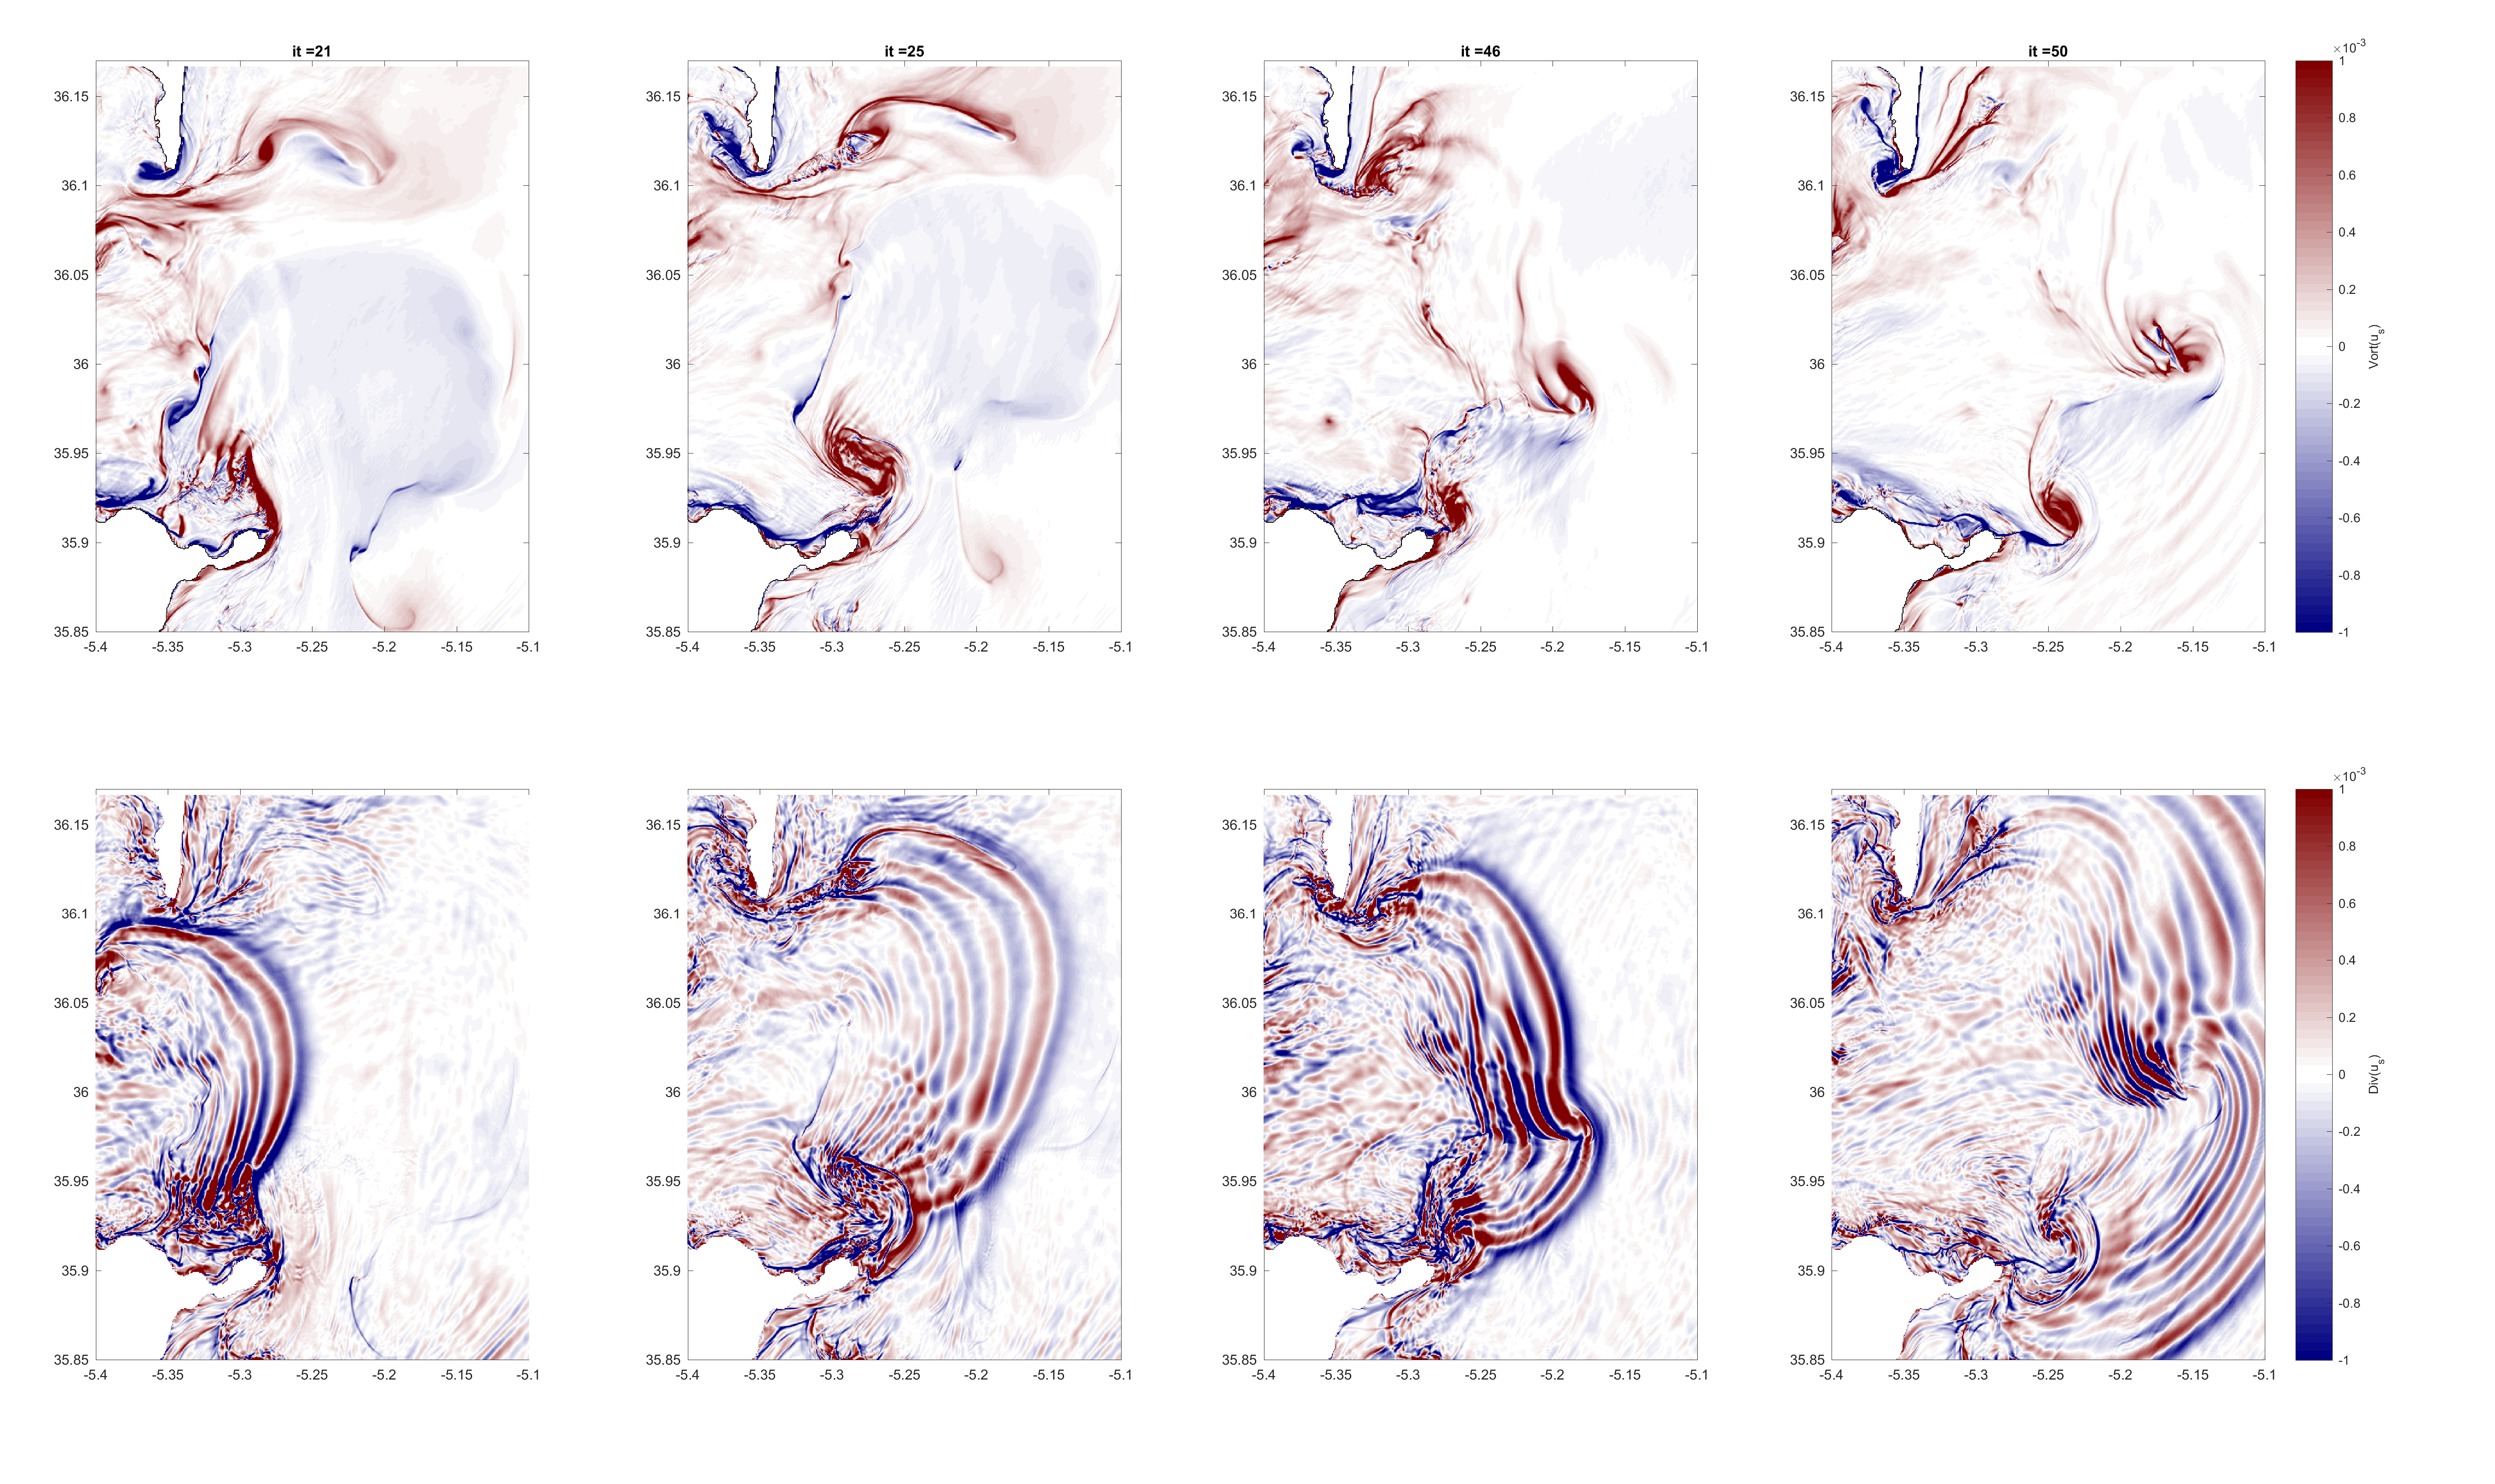
\includegraphics[width=\linewidth]{./GBR3D/FigTourbVE2.png}
%\end{subfigure}
 \caption {Divergence of surface current (upper row) at t=10.5H,12.5H, then 23H and 25H of simulation SimST,  and z-axis vorticity of surface current (lower row) for the same time.}
 \label{FigeddGBR3D}
\end{figure}

Solitary waves are generated at each tidal cycle at CS, except when there is no hydraulic jump, figure \ref{FigISWGBR3D} gives exemple of their propagation in Tarifa Narrows. Figure \ref{FigISWNT} also depicts the divergence of surface current but at the eastern exit of the Strait in inflow following a no-jump outflow. Can see that a train of solitary wave still ends up propagating in the alboran Sea, as the signal of the propagation of the baroclinic tide in figure \ref{FigISWNT}.b makes a more and more pronounced front with steeper isohaline that through the non-hydrostatic disperison balance with non-linearity devolves into a train of solitary waves. 

Compared to the upper row of figure \ref{FigeddGBR3D}, that also shows divergece of surface current but for inflows after hydraulic jump, those train of solitary waves are less extended than in case where tehre was hydraulic jump at CS. The lower row of figure shows the z-axis vorticity of surface currents at teh same time. The two inflow periods shown are separated by one tidal cycle. First two figure see a train of solitary waves exiting the strait, in figure of vorticity see that as it exists, a filament of positive vorticity is formed by interaction with the coast of Ceuta and develops into a cyclonic eddy.  detached from the coast. In \ref{FigeddGBR3D}.c one tidal cycle later the eddy is at 5.2$^o$W and 36$^o$N and thenleading waves of the next wave packet generated at this cycle are arriving at this position, disforming the shape of the packet, south part accelerated and north part decelareted, at the same time can see once again potential vorticity patch off of Ceuta. In \ref{FigeddGBR3D}.d this patch too has developped in a cyclonic eddy that propagates in the Alboran Sea while the interaction between the solitary waves and the previous cyclonic eddy has resulted in interference pattern in the wave packet. 


%However, even in case of no hydraulic jump, solitary waves end up  point the tide passing through the strait and through tarifa gives a signal at the surface that exiting the strait starts disppersing in a wave train, though not as extended. In the simulations, Always organised train with the leading wave being greater except when propagation in the ALboran Sea due to refraction on an eddy.

%This case is presented in figure \ref{FigeddGBR3D}, for simulation ...,  two rows of figure plotted the vorticity and divergence field of the surface currents. In figure \ref{FigeddGBR3D}.a wave packet arrives at exit of the Strait, in south part off of Ceuta, filament of positive vorticity. As the wave passes this area in \ref{FigeddGBR3D}.b the filament is now a cyclonic eddy detached from the coast. In \ref{FigeddGBR3D}.c one tidal cycle later the eddy is at 5.2$^o$W and 36$^o$N and thenleading waves of the next wave packet generated at this cycle are arriving at this position, disforming the shape of the packet, south part accelerated and north part decelareted, at the same time can see once again potential vorticity patch off of Ceuta. In \ref{FigeddGBR3D}.d this patch too has developped in a cyclonic eddy that propagates in the Alboran Sea while the interaction between the solitary waves and the previous cyclonic eddy has resulted in interference pattern in the wave packet. 

In the simulations, this process of generation of cyclonic eddy off of the coeast of Ceuta occurs each time solitary waves exit the srait,  The wave of the next tidal cycle gets diffracted on this eddy, creating interference in the train of solitary waves.



\subsubsection{Dynamic at Camarinal Sill, primary instabilities}


Along with the hydraulogical features of teh flow already discussed previously, figures \ref{FigHCN},\ref{FigHCS},and\ref{FigHCI}  indicate patches of high standard deviation of parameter Q. They are the most extended for all outflow cases and for the spring tide inflow, although the values for this latter case are not as high. High values of this parameter indicate oscillation of the value of parameter Q of greater amplitude, the highest are found for the two outflow case where hydraulic jump is detected (w-jump and s-jump), in the area west of CS at 5.79$^\text{o}$W and west of secondary bathymetric features in Tanger basin at 5.84$^\text{o}$W. There is also a signal at Espartel Sill, of greater standard deviation for the spring tide outflow.

Figure \ref{FigTSCS}.a superposes to the standard deviation to the singular vector of SVD of the 3D field of parameter Q computed during the outflow for the EOF that had the most high-frequencey variability in its eigenvector, associated with propagation of vortical structures (higher order EOF (not shown) have low frequency variability and structure associated with the regional flow itself). Can see that the contour of parameter Q$=5e-5m^2s^{-2}$ are located at same place as high standard deviation. See generation areas of vortexes are approximately centered around two longitudes 5.77$^\text{o}$W on the west slope of Camainal Sill and  5.84$^\text{o}$W on the west slope of secondary sills in Tanger Bassin. Figures \ref{FigTSCS}.b to e show the partial view of $\theta$-S diagram in part of the graph of med waters where every hydrological property at each grid point in the simulation for a given longitude. See that in b that at ...degrés still up at the sill have a repartition of med water masses alike that in figure \ref{Fig_Ini_WM3D}. then from c to d more and more homogenized along same latitude under the effect of mixing.

The 36.05 (yellow) points seen is a passage north of Camarinal along shallower depth of bathymetry and those waters are mixed to NACW west of this point.

\begin{figure}[!h]
% \centering
 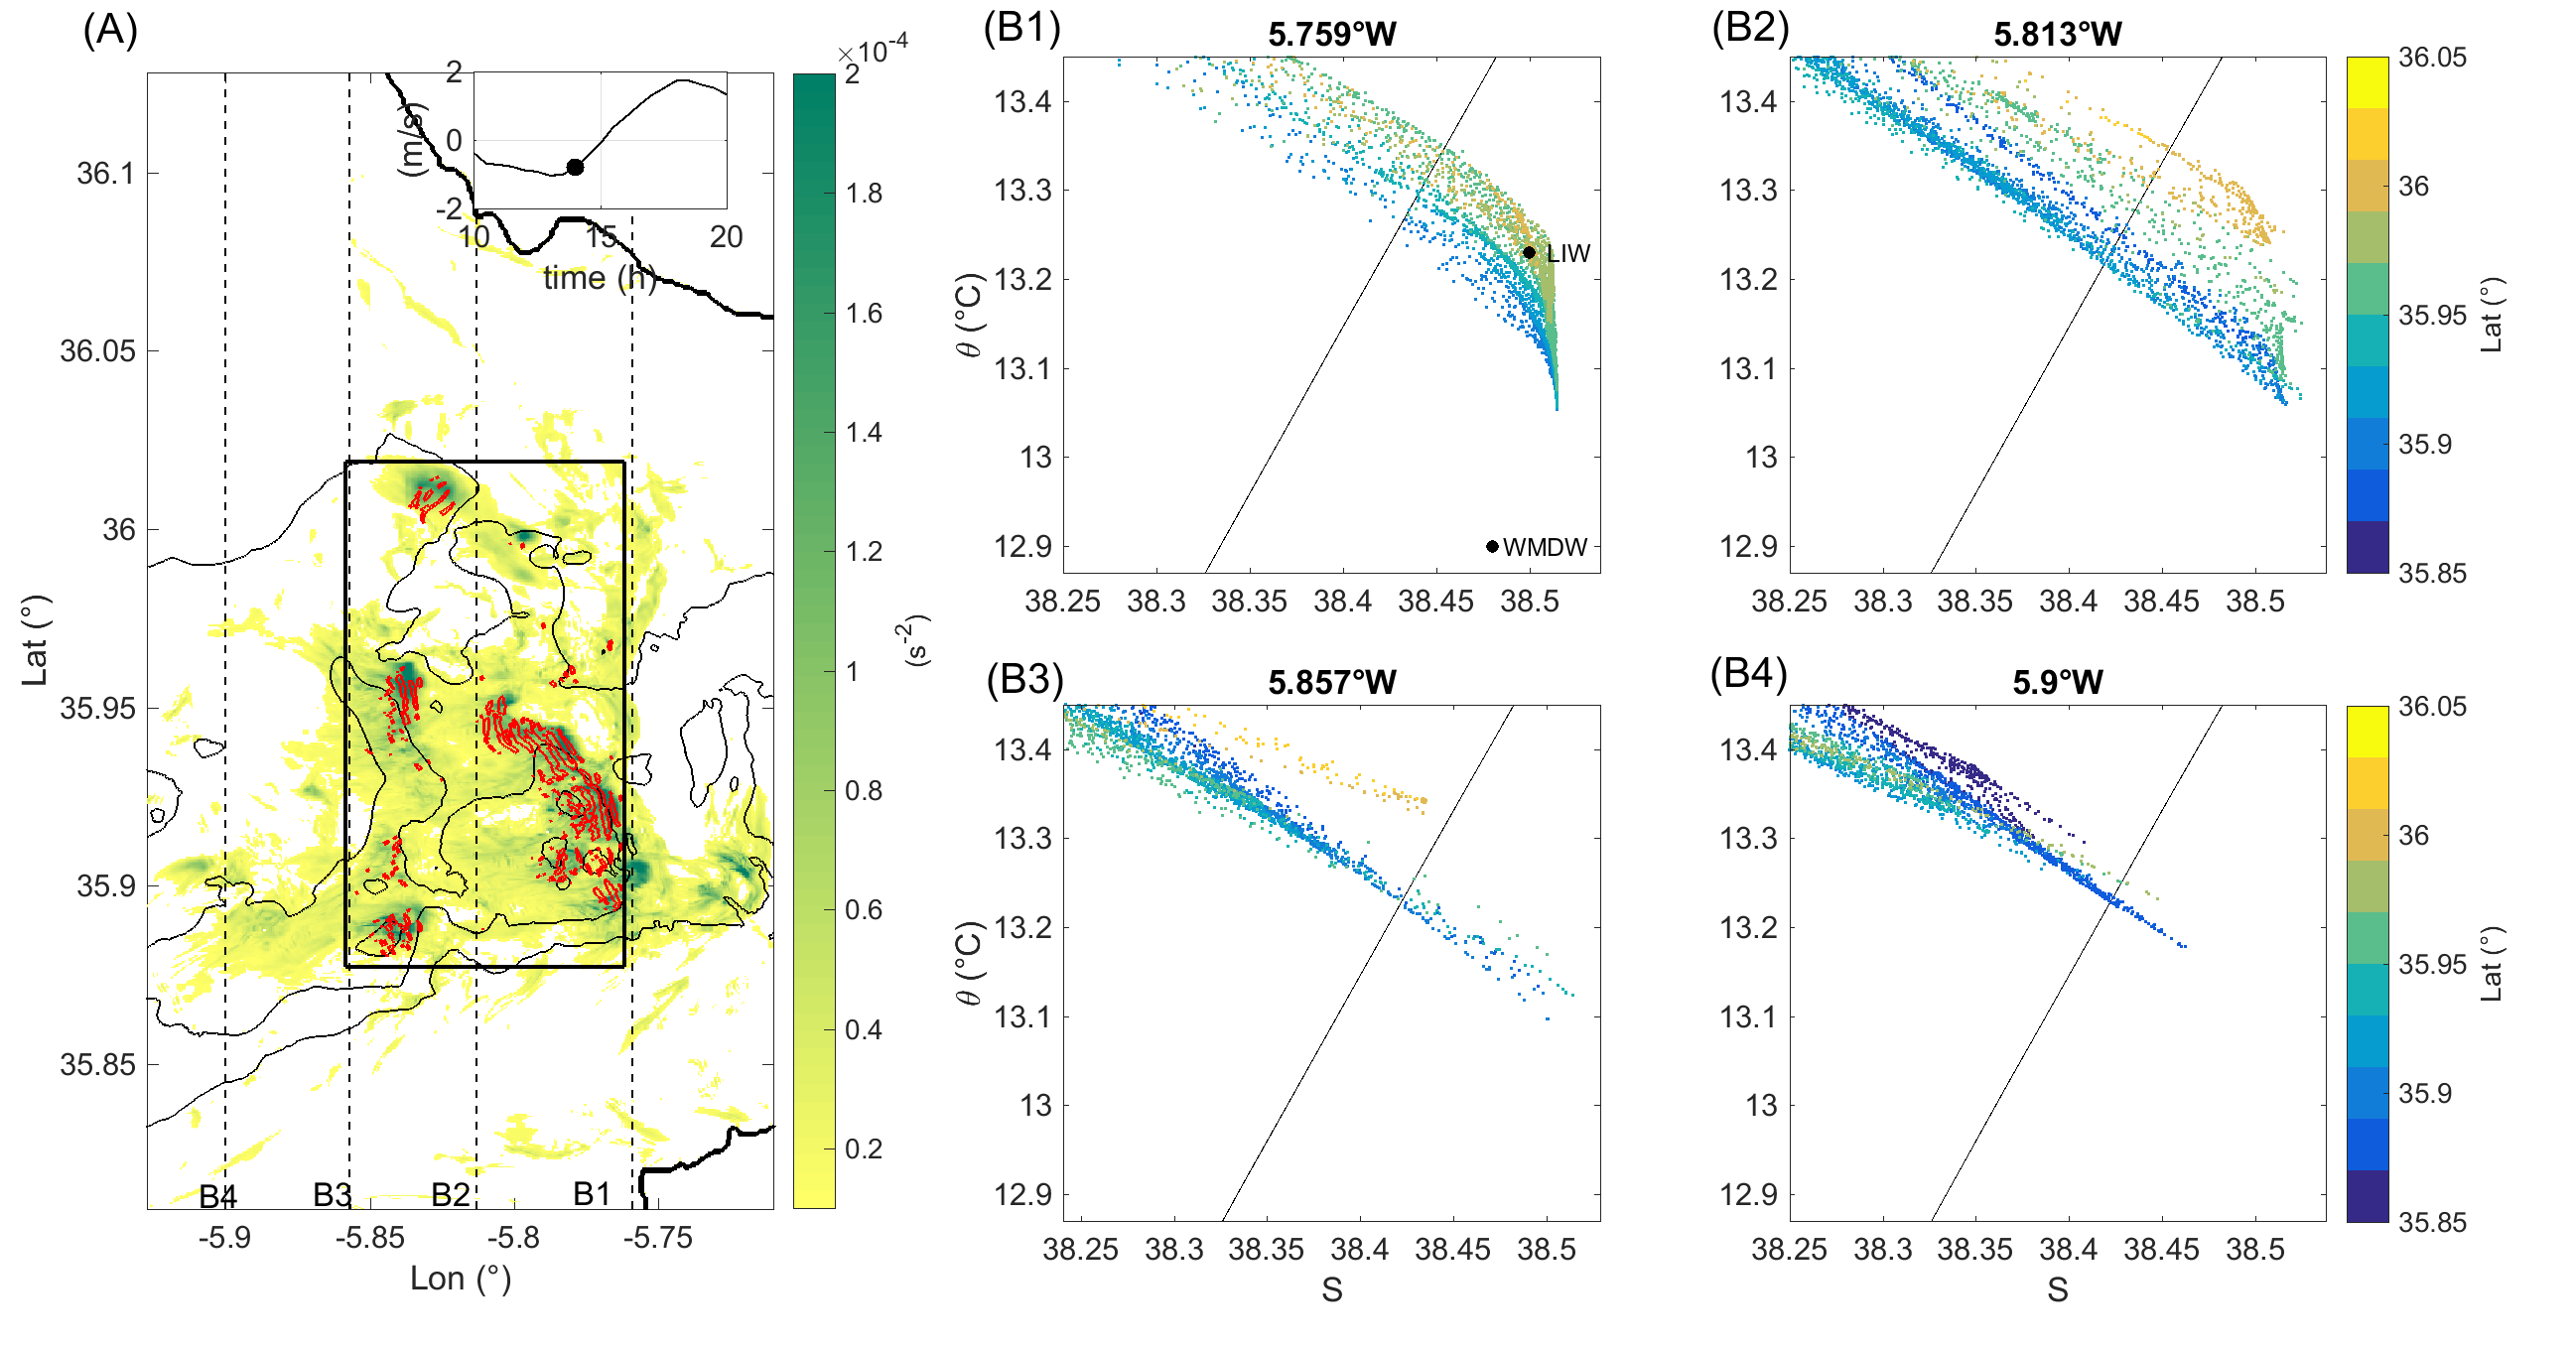
\includegraphics[width=\textwidth]{./GBR3D/TS_coupes_14H_VE2o.png}
 \caption {(a) Standard deviation of parameter Q over 30 mintues at t=14H in SimST (color) and trace of Q$=5$ from the high-frequency EOF of SVD performed in the rectangular black box during the outflow period. Black dashed lines indicate the longitude at which T,S diagrams are plotted. (b,c,d,e) T,S diagrams, zoomed in on area of Mediterranean watermasses. (Mettre LETTRES)}
 \label{FigTSCS}
\end{figure}


Now looking at the singular vectors of SVD for outflows of different strength of barotropic tidal currents . Figure \ref{FigEOFMIV}.a,b,c presents the EOF of parameter Q for the outflows of figures \ref{FigHCN},\ref{FigHCS},and\ref{FigHCI},along with vertical sections of salinity at the time of figure \ref{FigEOFMIV}d,e,f. Figure \ref{FigEOFMIV} g and h are histograms giving the height above seafoor and latitude of the grid points of the EOF for which Q$\geq 5e-5m^2/s^2$. On vertical sections, can see that the positive value of Q parammeter are associated with billow structures of salinity that develop in the gravity current along the west solpe of the Camarinal Sill. Those structures develop for each outflow case, but the wider distributions of height above seafloor and visualisation in the vertical section indicates the billows have greater radius in the hydraulic jumps cases, entraining more interfacial and atlantic waters into the mediterranean outflow. At this longitude where the instabilities are still developped, cores are not yet mixed in the simulation, can see as in the $\Theta$-S diagrams that the outflow is still heterogeneous.

The two hydraulic jump cases also differ, in the w-jump case, the start of the gravity current and the hydraulic jump are colocalised at this latitude, but not in the s-jump case, and 

while instabilities develop along the same areas in no-jump and s-jump case, in the w-jump case the hydralic jump and teh start of the gravity current are colocalised at all latitude as seen in the vertcial section, which adds a possible area of generation between 35.92$^\text{o}$N and 35.93$^\text{o}$N, downslope of the shallowest point of the sill where the flow of Mediterranean waters is not as strong for s-jump and no-jump cases.


\begin{figure}[!h]
% \centering
 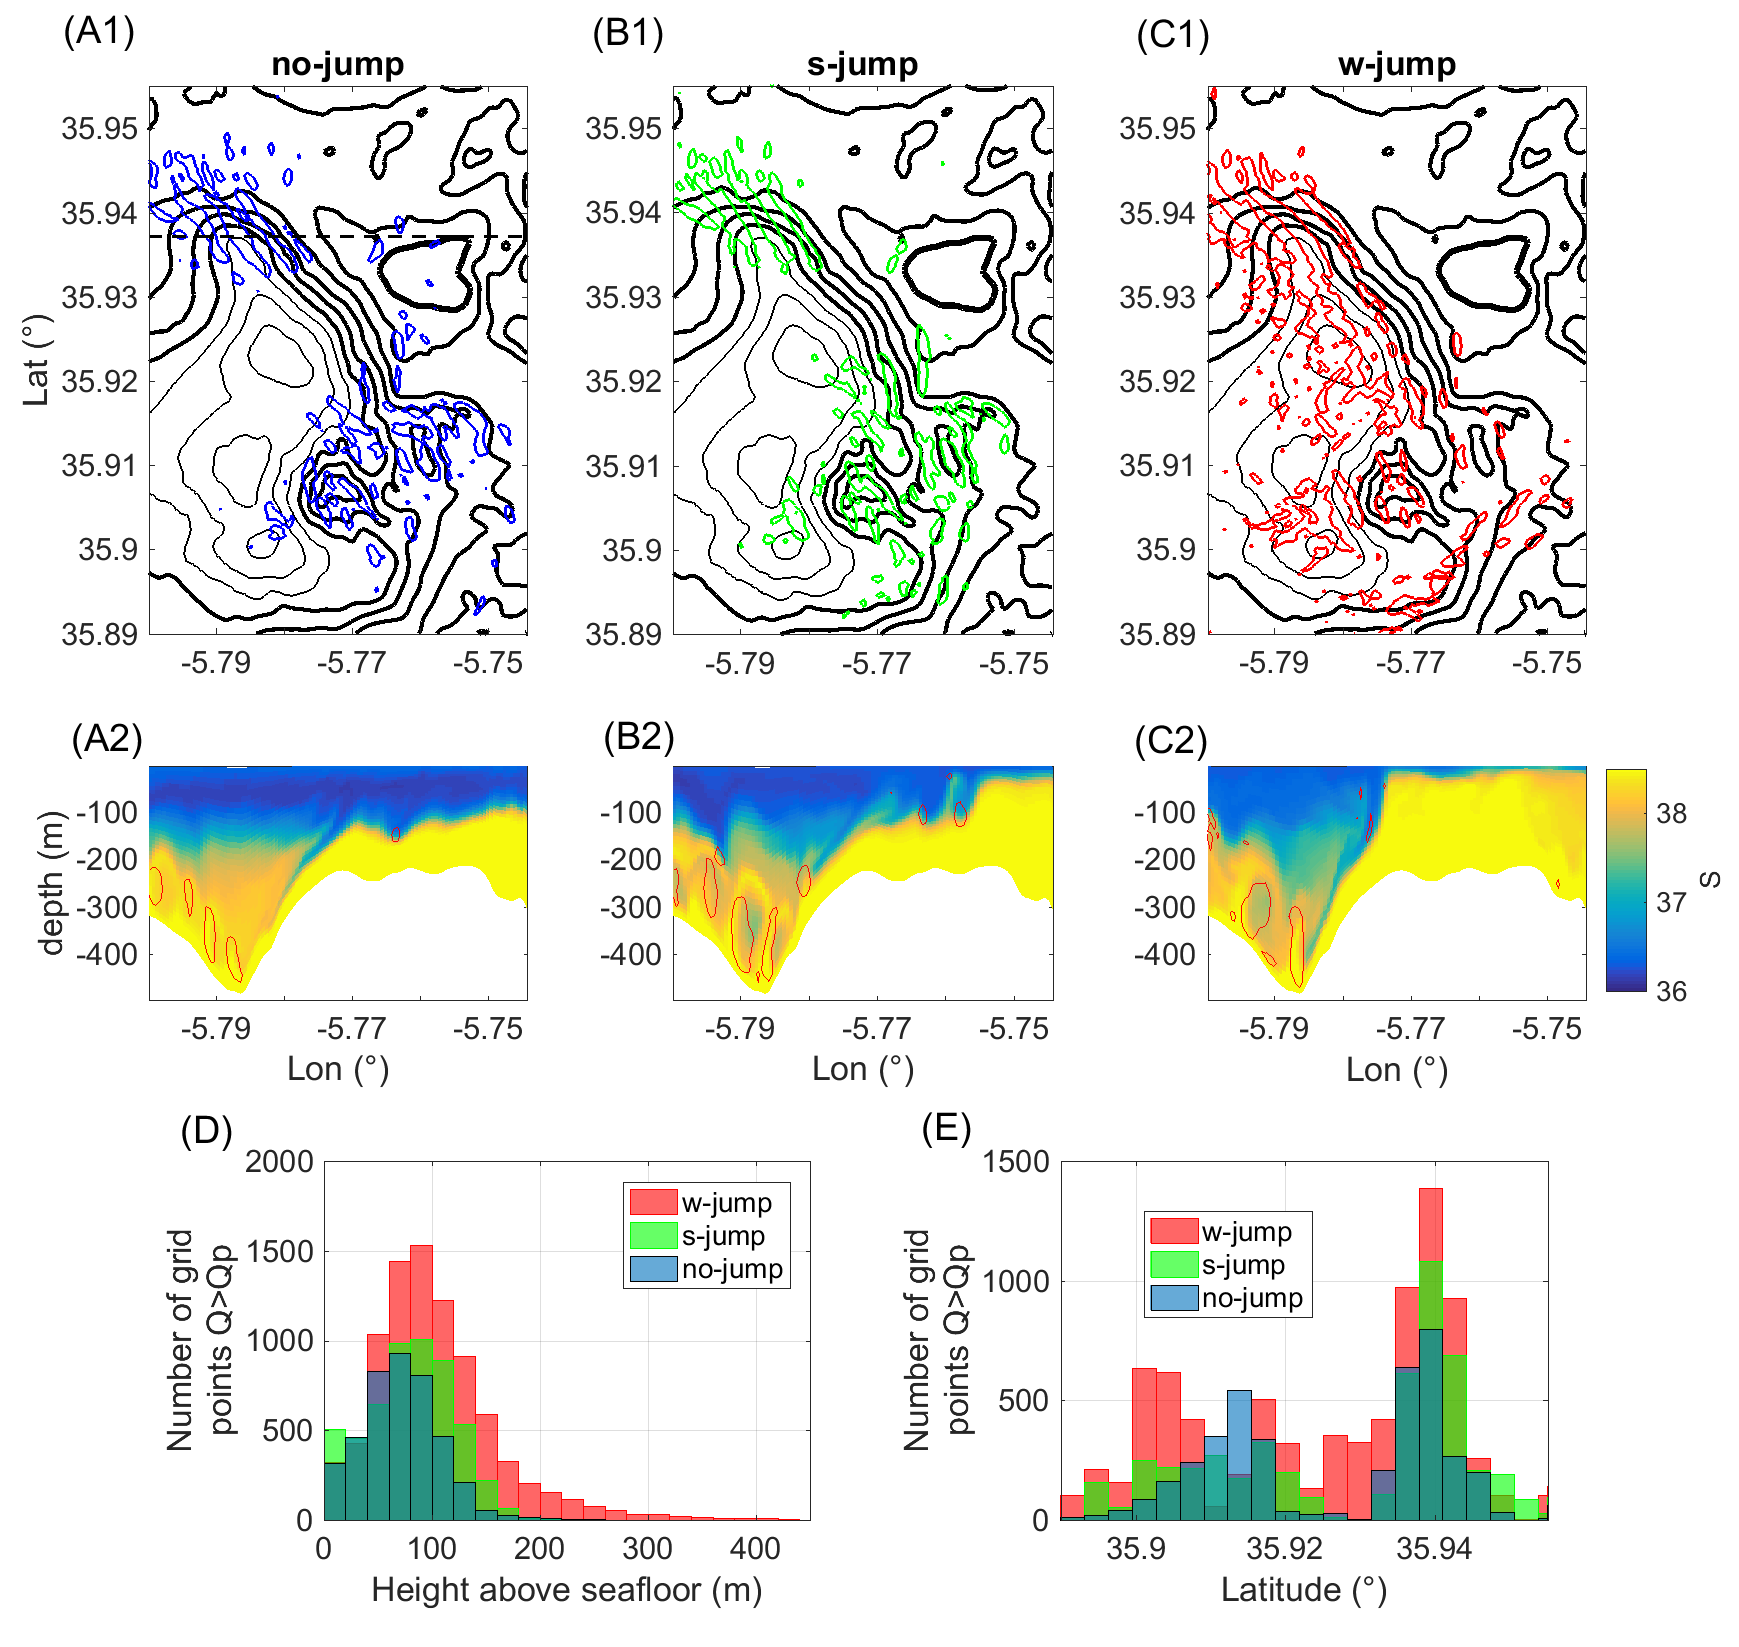
\includegraphics[width=\textwidth]{./GBR3D/EOF5_MIV_2D.png}
 \caption {(a,b,c) Contour of parameter Q$=5.10^{-5}$ in first high frequency EOF of SVD performed during outflow of figures \ref{FigHCN}.b,\ref{FigHCI} and \ref{FigHCS}.b respectively. and isobathes (black) (200m, thicker)  (250 to 450, thick) (500 to 600m, thin). (d,e,f) vertical section of salinity (color) and contour of Q-parameter $=5.10^{-5}$ at latitude $35.9372^\text{o}$ at the same time as figures \ref{FigHCN}.b,\ref{FigHCI} and \ref{FigHCS}.b respectively. (g) histogram of the height of the grid points of each EOF shown in a,b and c above the seafloar. (h) histogram of the latitude of the grid points of each EOF shown in a,b and c above the seafloar. }
 \label{FigEOFMIV}
\end{figure}


(phrase plutot pour conclusion?) Can easily see that the configuartion of the flow at CS, by being the first passage of the Med waters, will affect the hydrological properties, first by the volume of med waters that can flow west of the sill at each outflow, second by how much atlantic waters are entrained. A point that was not studied here is that not only those hydraulogical characteristics but also dynamical properties of the ouflow.


\subparagraph{Closure scheme}

Now look at four other simulations, three use Smagorinsky turbulent scheme with different coefficients. One is using GLS K-$\epsilon$. In figure \ref{Fig3Dsch}.a,c,e,g, vertical section of salinity during the first outflow which is in a no-jump case, with Richardson gradient number $Ri$ and Q parameter indicated. $Ri$ is calculated for a field averaged for a half hour to filter out the propagating structures.

Figure \ref{Fig3Dsch}.b,d,f,h the averaged salinity in med (b,f) and atl layer(d,h),east (f,h) and west (b,d) of Camarinal Sill. Note that this is averaged value, as shown in figure and can be seen in the vertical sections the outflow is not homogeneous at this longitude yet.

In vertical sections, can see that the area of $Ri=0.25$ starts at 5.77$^\text{o}$ for all four simulations, indicating shear instabilities could develop from this point in the gravity current. This is the case for all simulations but SimIT-S1, for which they only develop downflow of an intrusion of atlantic waters at 5.783$^\text{o}$W. 


While the width of the Med vein as it begins to go downslope of Camarinal as salty water is the same, in simulations 1 and 2 instabilities are earlier in the jump and bring more atl waters as the core or billows are advected downslope, resulting in more atl water being integrated to the med outflow at the passage of CS. Figure gives the average salinity of the med outflow taken at lon ... averaged over all latitude (med outflow defined by all parcels of salinity superior to interface smlinity...).



%Case S0.001 instabilities devlop from the inset of the jump at approx 5.77 deg and the billows contain less salty waters, ie the signal of atl surface water in the med outflow will be stronger in this simulation.


The salinity of the mediterranean outflow seems more sensible to the area where generation occurs, even if the stability condition is the same along the gravity current, in SimIT-S1the first instabilities are simulated further down the slope. In contrast Case S0.001 instabilities devlop from the inset of the jump at approx 5.77 deg and the billows contain less salty waters, ie the signal of atl surface water in the med outflow will be stronger in this simulation.


%While the width of the Med vein as it begins to go downslope of Camarinal as salty water is the same, in simulations 1 and 2 instabilities are earlier in the jump and bring more atl waters as the core or billows are advected downslope, resulting in more atl water being integrated to the med outflow at the passage of CS. Figure gives the average salinity of the med outflow taken at lon ... averaged over all latitude (med outflow defined by all parcels of salinity superior to interface smlinity...).

%Looking at condiftions for the instability development, richardosn number (computed on 1h averaged field to filter the billows) is below 0.25 for each simulation, however, looking more in detail the shear and stratification, stratification is more or less teh same but shear is lesser in 3.

This is counterintuitive as SimIT-S1 has a greater diffusivity and viscosity, this acts without instabilitied for exemple like east of the sill in figure with enhancing mixing in the haloclyne with surafce waters becoming saltier and deep waters becoming less salty.

Kepsilon on the other hand see less developped roll of salinity although the instabilities begin at ... On average this seems to lead to a slightly less salty mediterranean vein.

%Note that this is averaged value, as shown in figure and can be seen in the vertical section the outflow is not homogeneous at this longitude yet.


\begin{figure}[!h]
% \centering
 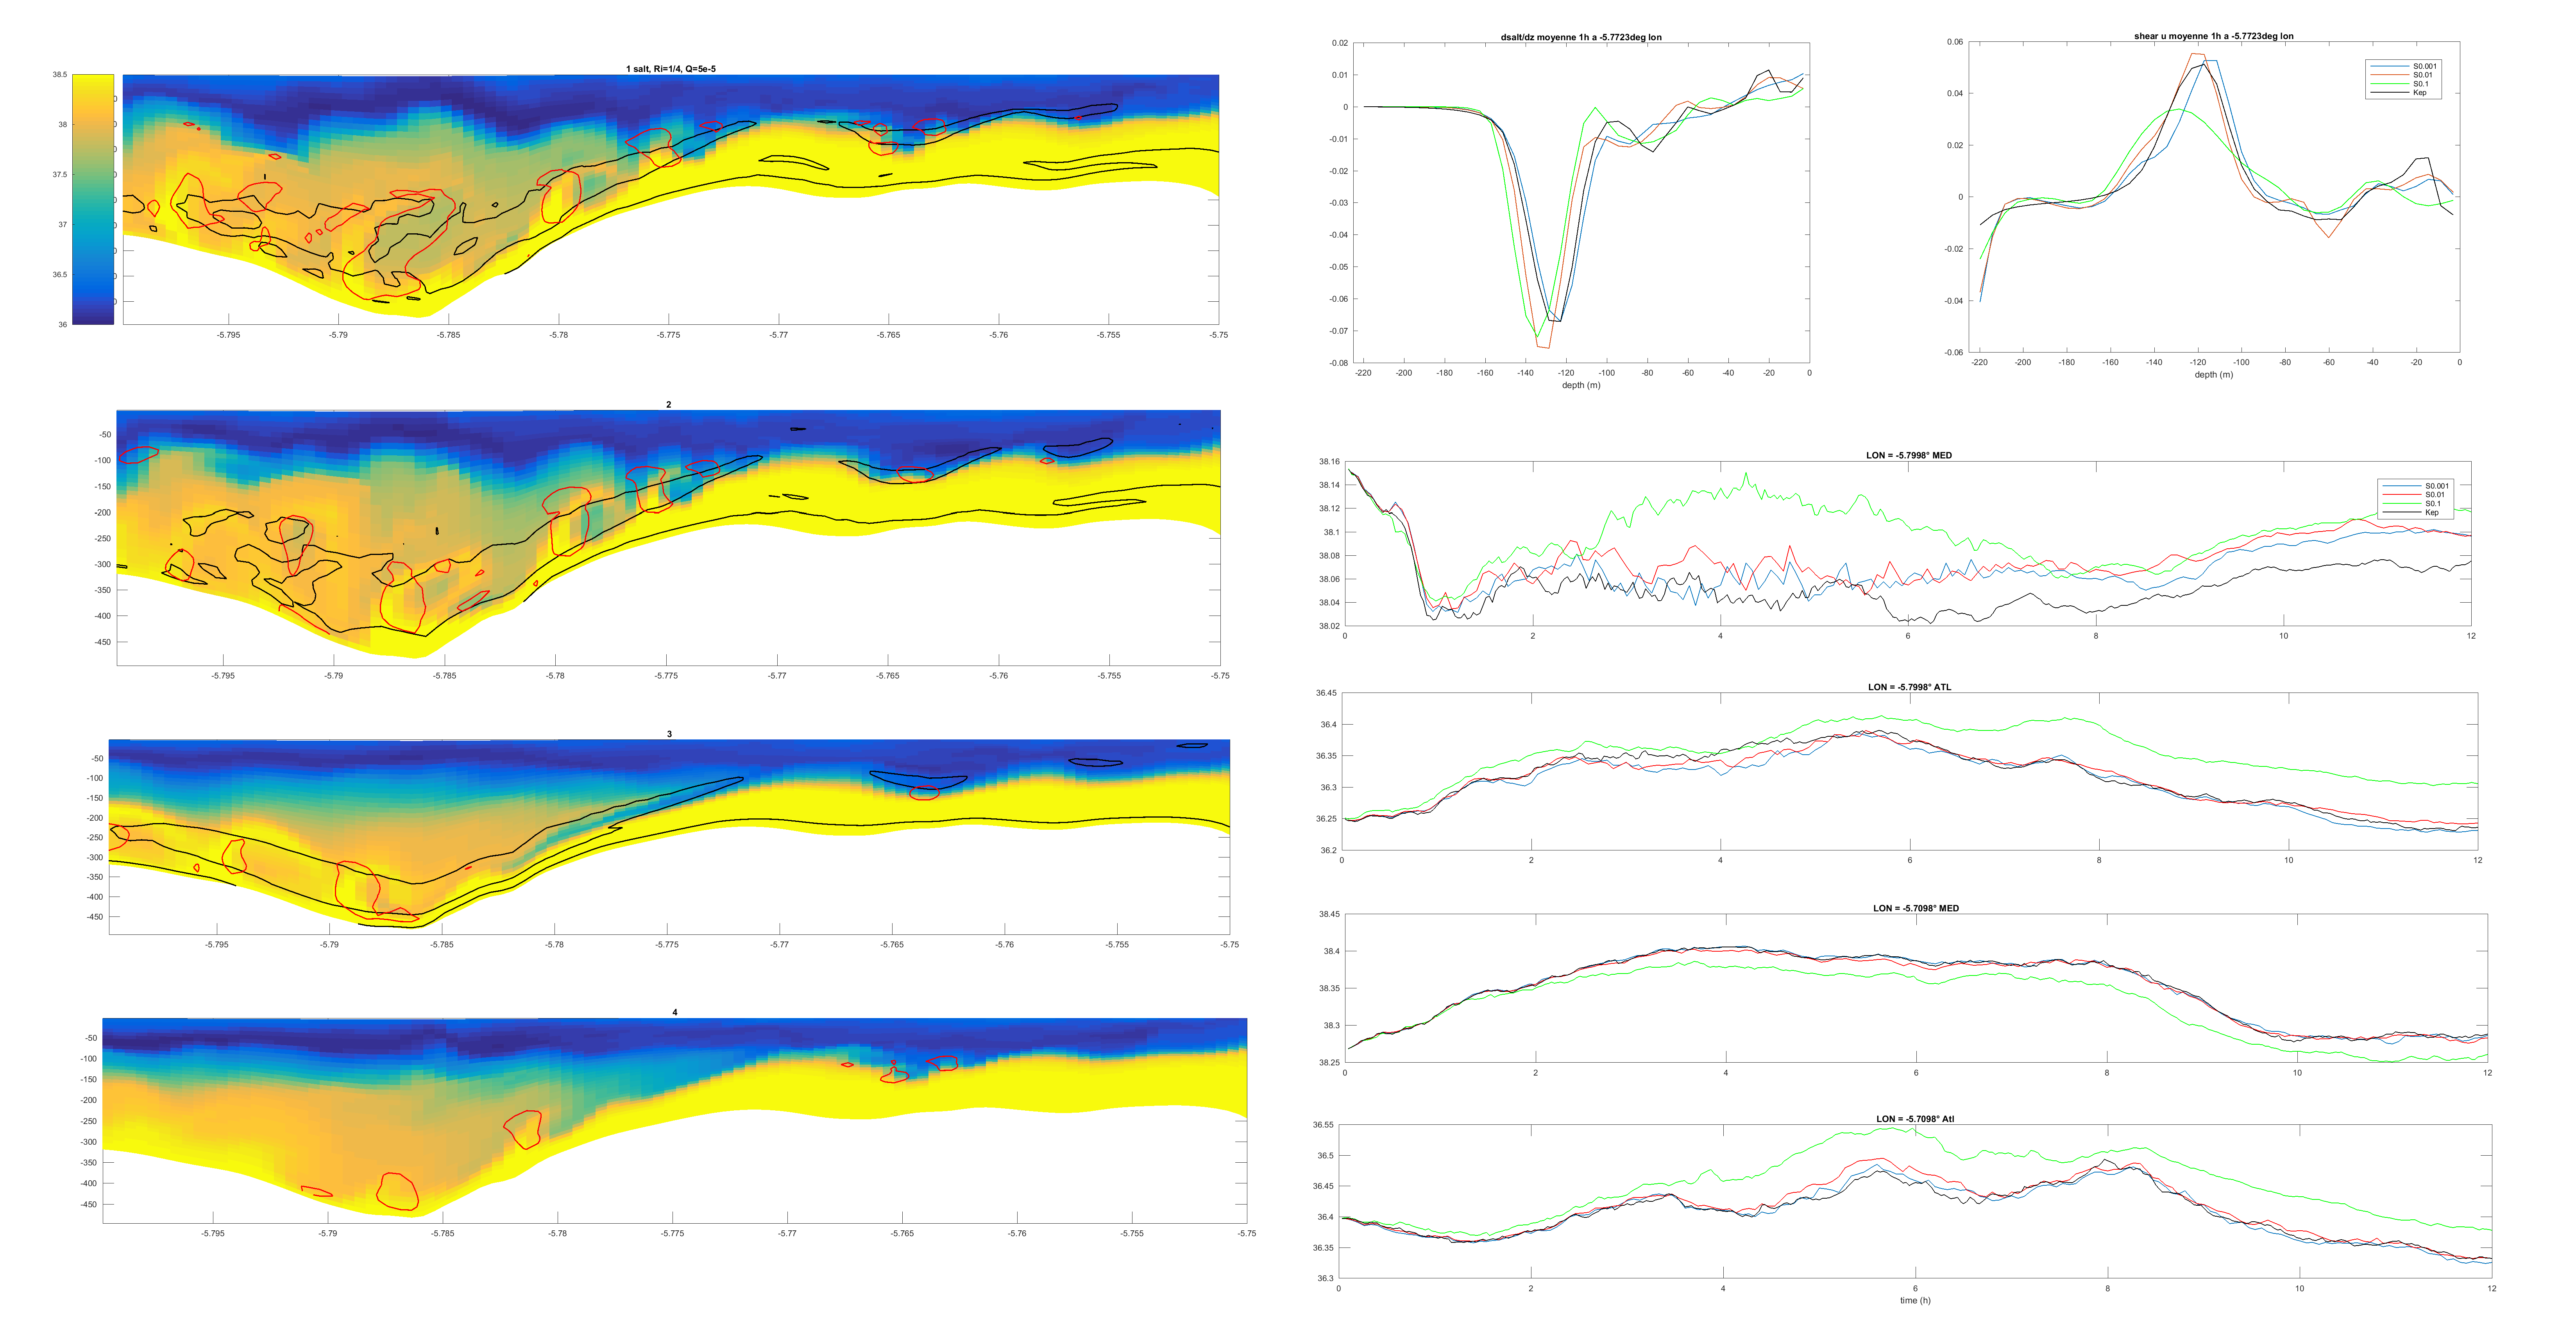
\includegraphics[width=\textwidth]{./GBR3D/Figsmago.png}
 \caption {Vertical section of salinity (color) and contour of $Q=5.10^{-5}$ (red) and Richardson gradient number $=025$ (black) at lat = $35.9372^o$ in simulations SimIT-S001,SimIT-S01,SimIT-S1 and SimIT-Kep IES at t=4h of simulation. time  (1:S0.001  2:S0.01  3:S0.1 4:Kep)(Rajouter une évolution de ubar!!! sur s0.001)}
 \label{Fig3Dsch}
\end{figure}

%-------------------------------------------------------------------------------------
\subsection{Discussion}

Analysed the criticality of the flow in realistic oceanic simulation of the Starit of Gibraltar. See no permanent supercritical flow accross the simulations, only intermitent with the tidal cycle, ith location and extension of the area of supercritical flow depending on the strength of the barotropic currents.

In outflow when both atl and med layers are critical, hydraulic jump, which position is either over the shallowest part of the sill, or over its western slope. This hydraulic jump evolves into train of solitary waves at the tidal bascule, that exits teh strait into the Alboran Sea. Even for tidal cycle for which the flow over the sill is not critical and there is no formation of hydraulic jump, the non-linearity of the propagation of the barotropic tidal signal in the eastern part of the strait devolves into a less extended train of solitary waves propagating into the Alboran Sea.

At each simulated tidal cycle, a cyclonic eddy is formed of the coast of Ceuta in teh southern part of the eastern exit of the Strait. This eddy is advected by teh flow in th Alboran Sea and interacts with the train of solitary waves.

Finally, simulkation is well-enough resolved that primary istability of shear are resolved. They are generated at ... and are advected with the shear between med outflow and atlantic waters as was the case in 2D simulation of Hilt 2020, with mixing occuring downflow of those area of propagation of those primary instabilities as they are simulated. See that the tidal regime also impacts extent of area of generation and strength of such instabilities. 

However, it is important to note that simulation only represents the beginning of the mixing by turbulent processes, and while the generation process is simulated, where they are generated and their evolution is depednant on the turbulence closure scheme used. In particlular, a higher coefficient of the Smagorinsky means higher value of mixing coefficient, but teh simulated features in the hydraulic jump are not as efficient in incorporating atlantic waters into the med outflow, resulting in a saltier med outflow.








(notes conclusions : strength of the barotropic tide makes for varying cases of hydraulogy of the flow of the two-layer exchange. hyd jump detection seems to be linked here to the criticality of the atl layer, and gives surface signature. it occures for all cases here, although the neap inflow case still has a 1m/s barotropic current while the neap outflow was at 0.5m/s and weaker inflow may exist in nature and result in different situation. ((The most interesting hyd jump are the outflows where they are associated  )). criticality for the inflows in area of TN is linked to both the strength of the barotropic current wich pilots the extent of the flow in the nothern area and the presence of propagating solitary wave which induces critical flow in south part.

In particular wind friction(?) is known to impact the flow of the atlantic layer in tarifa narrows and ... . as well, does not represent the alboran gyre that commands dynamic at the eastern exit of the strait, in peuclar its current (especially the atlantic jet) could advect the eddy generated by soliton outside the border of the simulations domain and cause the solitary wvae train to be refracted in other shapes. As well all trains observed in simulations are organised with the leading wave having the greater amplitude (not shown (ou pourrait voir avec champ profondeur de l'interface ???)), whoch according to ... is not usually the case.

strong outflows are associated  with areas of enhanced generation/propagation of vortices(avec part d'après sait), they are essentially axe of rotation is horizontal and are associated with billows structure of tracers like salinity. water mass properties change between areas where billows are .one crucial point is that the way there are represented in the code will pilot the mixing between atl and med waters, and it can change drastically with turbulence scheme used.


\subsection{Conclusion}

have looked into the variabilty in neap-spring tidal cycle of hydraulic control and other features in high resolution non hydrostatic simulation of the strait of gibraltar. this simulation features the expected internal solitary wave propagation, as well as billows in the lee of CS that seem linked to the ones that have been observed by ... . In simulations, these billows are associated with high value of paramater Q that is used as proxy for their deetction and analysis. Those billows are generated at interface of med and atl waters and advected by the med outflow.   they could also be present at secondary reliefs in tanger basin and at espartel sill. They are present during outflows of all intensity, but their repartition will change with intesity of tidal currents. They have a role in the way the med water is mixed, with changes of hydraulogical features of the med vein, and in simulation the way this mixing occurs is sensible to the dynamic of the instabilities that is piloted by the turbulent dissipation scheme.



Gib :
More mixing expected west of CS than east... Mediterranean vein also mixed in Gulf of Cadiz.

Spatial (here) and temporal variability can be studied... See area of expected billows extends more in south path than northern one. (Millot 20?? : Mixing not the same north or south)



blabla LES..

High resolution modelling of key areas open possibilities in parametrisation, imbricated models etc... tool that needs to be more studied 

The prevalance/importance of numerical dissipation associated with advection scheme needs to be carefully assessed, in particular here the structure of the primary instabilities and how it is resolved/behaves is key at 

Interest for global models but also for field studies as to chose precisely areas. Although need a framework that make comparison of mixing measured across this medium more easy (Gregg review..)







